\documentclass[]{article}
\usepackage{amsmath}
\usepackage{amsfonts}
\usepackage{amssymb}
\usepackage{hyperref}
\usepackage{gensymb}
\usepackage{graphicx}
\usepackage{svg}
\usepackage{bbding}
\usepackage{mathtools}
\usepackage{centernot} % not parallel, etc.
\usepackage{lmodern}
\usepackage{morewrites}
\usepackage{xcolor,sectsty} % colorful sections
\usepackage[left=10mm, top=10mm, right=10mm, bottom=20mm, nohead]{geometry}
%\usepackage{bigints}
\usepackage{dsfont} %mathbb 1
\usepackage{esint} % beatiful integrals
\usepackage[arrowdel]{physics}


\DeclareFontFamily{OMX}{lmex}{}
\DeclareFontShape{OMX}{lmex}{m}{n}{<-> lmex10}{}


%colors of sections
\definecolor{secfont}{RGB}{46,116,181}
\definecolor{subfont}{RGB}{146,23,57}
\definecolor{parfont}{RGB}{19,127,43}
\definecolor{subparfont}{RGB}{7,11,100}

\subsectionfont{\color{subfont}}
\sectionfont{\color{secfont}}
\paragraphfont{\color{parfont}}
\subparagraphfont{\color{subparfont}}

%\usepackage{babel}[english]
%opening
\title{114246 - Electromagnetism and Electrodynamics}
\author{Adi Nusser}
% Lidow 612
% Landau Lifshitz Classical theory of fields, Electordynamics
% Jackson Electrodynamics 
% Electromagnetism in a nutshell

\parindent=0em
\begin{document}


\maketitle

\begin{abstract}

\end{abstract}

%\tableofcontents
\section{Introduction}
In this course we use CGS system. Force between two charges is
$$\va{F} = \frac{q_1q_2}{\vb{r}^2}\vu{r}$$
The unit of charge is statcoulomb, or esu.

Field around charge $q$ is
$$\va{E} = \frac{\va{F}}{q'}= \frac{q}{\vb{r}^2}\vu{r}$$
Then force can be written as $$\va{F} = q' \va{E}$$

\paragraph{Principle of linearity (superposition)}
If we have some frame of reference we can rewrite force as
$$\va{F}_1 = \frac{q'q_1}{\abs{\va{r'}-\va{r}_1}^3}\qty(\va{r}-\va{r'})$$
And fields can be summed as following:
$$\va{E} = \sum_{i=1}^N E_i = \sum_{i=1}^N \frac{q_i(\va{r'}-\va{r}_i)}{\abs{\va{r'}-\va{r}_i}^3}$$

If charge is continuous define
$$\rho(\va{r}) = \frac{\Delta q}{\Delta V}$$
field turns into integral:
$$\vec{E}(\va{r}) = \int \dd[3]{\vb{r'}}  \rho(\va{r'}) \frac{\qty(\va{r}-\va{r'})}{|\va{r}-\va{r'}|^3}$$
\paragraph{Potential}
$$\vec{E} = \frac{q\va{r}}{\vb{r}^2} = -\grad{\frac{q}{r}} $$
For some frame of reference
$$\vec{E} = \frac{q(\va{r}-\va{r'})}{|\va{r}-\va{r'}|^3} = -\grad\frac{q}{|\va{r}-\va{r'}|} = -\grad \Phi$$
\paragraph{Gradient, divergence and Laplacian in spherical coordinates}
$$\grad{f(r, \theta, \phi) } = \vu{r} \pdv{f}{x} + \vu{\theta} \frac{1}{r} \pdv{f}{\theta} + \hat{\phi} \pdv{f}{\phi} \frac{1}{r \sin \theta}$$
$$\div{\va{A} (r,\theta, \phi) } = \frac{1}{r^2} \pdv{r} (\vb{r}^2 A_r) + \frac{1}{r\sin \theta}\pdv{\theta}  (\sin \theta A_\theta) + \frac{1}{r \sin \theta} \pdv{ A_\phi}{\phi}$$
\paragraph{Continuous case}

$$\vec{E}\qty(\va{r}) = \int \dd[3]{r'} \rho\qty(\va{r'}) \frac{\qty(\va{r}-\va{r'})}{\abs{\va{r}-\va{r'}}^3} = -\grad \int \frac{\dd[3]{\vb{r'}} \rho(\vb{r'})}{\abs{\va{r}-\va{r'}}} $$
And
$$\Phi = \int \frac{\dd[3]{\vb{r'}} \rho\qty(\vb{r'})}{\abs{\va{r}-\va{r'}}}$$
\paragraph{Gauss theorem}
$$\int\limits_V \dd[3]{\vb{r}}\div {\va{A} \qty(\vb{r})} = \oint \va{A} \vdot \dd{\va{s}} = \oint \vb{A}_n \dd{s}$$

Lets apply Gauss theorem on electric field of point charge in origin:
$$\div{\va{E}} = \div{ \frac{q \va{r}}{\vb{r}^3}}$$
Then
$$\div{\va{E}} = -\laplacian{\frac{q}{r}} $$
If $r\neq 0$,
$$\div{\va{E}} = q \grad {\frac{\va{r}}{\vb{r}^3}} = q \grad {\frac{\vu{r}}{\vb{r}^2} }= \frac{q}{\vb{r}^2} \pdv{r} \left( \vb{r}^2 \frac{1}{\vb{r}^2}\right) = 0 $$

By applying Gauss law:
$$\int\limits_V \dd[3]{\vb{r}} \div{\va{E}} = \oint \va{E} \dd{\va{s}} = \int \dd{\Omega}  \frac{q\vu{R}}{\vb{R}^2} \vdot \va{R} \vdot \vb{R}^2 = q\oint \dd{\Omega}  = 4\pi q$$
Which is right for a ball of any radius, in particular,  $R \to 0$. Thus
$$\div{\va{E}} = 0$$
while
$$\int\limits_{V_\epsilon} \div{\va{E}} \dd[3]{\vb{r}}= 4\pi q$$ 
\paragraph{Delta function}
Lets define 
$$ \begin{cases}
\delta^D = 0 & x\neq0\\
\int\limits_{x\in V} \delta^D(x) \dd{x} = 1
\end{cases}$$
We can define it as limit of 
$$F_\Delta = \begin{cases}
\frac{1}{\Delta} & -\frac{\Delta}{2} < x<  \frac{\Delta}{2}  \\
0 & otherwise
\end{cases}$$
Then $\lim_{\Delta\to 0} F_\Delta = \delta^D$.
\paragraph{Potential of point charge}
For a charge in point $\vb{r}_a$:
$$\div{\va{E}} = 4\pi q \delta^D \qty(\va{r} - \va{r}_a)$$
And for a couple of charges
$$\div{\va{E}} = 4\pi \sum_a q_a \delta^D \qty(\va{r} - \va{r}_a)$$
Then we can define dencity of charge for a point charge as
$$\rho\qty(\va{r}) =  \sum_a q_a \delta^D \qty(\va{r} - \va{r}_a)$$
And then in both cases
$$\div{\va{E}} = 4\pi \rho \qty(\va{r})$$
Since
$$\vec{E} = -\grad {\Phi}$$
$$\grad{ \left(-\grad{ \Phi}\right) }= 4\pi \rho$$
Which means
$$\laplacian{\Phi} = -4\pi \rho$$
which is Poisson equation. For bound conditions of $\phi, E \stackrel{r \to \infty}{\to} 0$ solution is $E = q\frac{\vu{r}}{\vb{r}^2}$.
\subsection{Bound conditions}
\paragraph{Direchlet bound conditions}
$\Phi = \Phi_S\qty(\va{r})$
for $r \in S$.
\paragraph{Neumann bound condtions}
We have $E_n$ on $S$.
\subsection{Example of Solutions}
Suppose we have Dirichlet bound conditions: $\Phi_S=0$. Obvious solution is $\Phi=\rho=0$

Lets show it's unique solution:
$$\int\limits_V E^2 \dd[3]{\vb{r}} = \int |\grad \Phi |^2 \dd[3]{\vb{r}} $$
$$|\nabla \Phi |^2 = \grad{\Phi} \vdot \grad{\Phi} = \grad\left(\Phi \vdot \grad{\Phi}\right) - \Phi \laplacian{\Phi}  = \grad\left(\Phi \vdot \grad{\Phi}\right)$$
$$\int\limits_V E^2 \dd[3]{\vb{r}} = \int \grad\left(\Phi \vdot \grad{\Phi}\right) \dd[3]{\vb{r}} \stackrel{\text{Gauss}}{=} \oint \Phi \vdot \grad{\Phi} \vdot \dd{\va{s}} = 0 $$
Thus $E=0$ and $\Phi=0$.
\paragraph{General case}
In general case $\laplacian{\Phi} = - 4\pi q$. Suppose we have bound conditions $\Phi = \Phi_S \neq 0$. Suppose we have two solutions $\Phi_1$, $\Phi_2$. 

Take a look at $\Phi = \Phi_1 -\Phi_2$, which has boundary conditions $\Phi_1-\Phi_2=\Phi_S-\Phi_S=0$, thus solutions are equal, from previous paragraph.
\paragraph{Neumann bound conditions}
Instead of $\Phi$ we now have $E_n =-\grad{\Phi} \vdot \vu{n} = 0 $.
$$\int\limits_V E^2 \dd[3]{\vb{r}} = \int \grad\left(\Phi \vdot \grad{\Phi}\right) \dd[3]{\vb{r}} \stackrel{\text{Gauss}}{=} \oint \Phi \vdot \grad{\Phi} \vdot \dd{\va{s}} = \oint \Phi \vdot \underbrace{\grad{\Phi} \vdot \vu{n}}_{-E_n} \dd{s} =  0 $$
Thus $E=0$. Note that $E_n$ determines $E_t$.
\paragraph{Earnshaw theorem}
If in some volume $\rho=0$, then there is no local  maximum or minimum of potential in this volume, since then $\grad{\Phi} = 0$ and either $\laplacian{\Phi} > 0$ or $\laplacian{\Phi} < 0$, but $\laplacian{\Phi} = \rho = 0$
\subsection{Methods of solutions of Poisson equation}
\paragraph{Method of image charges}

Suppose we have infinite grounded plane and a point charge in distance $a$ from it. The bound condition is $\phi(x=0,y,z) = 0$ And the potential of point charge is
$\laplacian{\Phi} = -4\pi q \delta \qty(\va{r} - \va{r}_0)$

The way to solve this kind of problems is to add imaginary charge such that we get zero potential on bound (e.g., symmetrically with opposite charge).

If we have two such charges:
$$\Phi = \frac{q}{(x-a)^2+y^2+z^2} -  \frac{q}{(x+a)^2+y^2+z^2}$$
This fulfills bound conditions:
 $$\phi(x=0,y,z) = \frac{q}{a^2+y^2+z^2} -  \frac{q}{a^2+y^2+z^2}= 0$$
 
 Denote density of charge on plane as $\sigma$, then $\dd{q} = \sigma \dd{s}$. If this case force between plane and charge is $\abs{\frac{\sigma q \dd{s}}{R^2}}$
 
 How do we find $\sigma$? From Gauss law
 $$\oint \vec{E} \cdot \dd{s} = 4\pi \int\limits_V \rho \dd[3]{\vb{r}}$$
 $$-|E_n|\dd{s} = 4\pi \sigma \dd{s}$$
 $$4\pi \sigma = E_n$$
 
 \subsection{Green function}
 Suppose we have a unit charge in point $\va{r'}$. Then potential is $\Phi_{\va{r'}}$ such that $\Delta \Phi = -4\pi \delta (\va{r} - \va{r'}) $.
 $$G\qty(\va{r}, \va{r'}) = \Phi_{\va{r'}}$$
 Thus
 $$ \laplacian{G\qty(\va{r}, \va{r'})} = -4\pi \delta \qty(\va{r} - \va{r'}) $$
 Then we can write $G$ as
 $$G\qty(\va{r}, \va{r'} ) = \frac{1}{\abs{r-r'}} + F\qty(\va{r}, \va{r'} )$$ 
 And $F$ guaranties bound conditions, while $ \laplacian{F} = 0$.
 
 \paragraph{Bound conditions}
 \begin{enumerate}
 	\item $G\qty(\va{r}, \va{r'}) = 0$.for bound $S$.
 	\item $ \pdv{\vu{n}}G(\va{r}, \va{r'}) = -\frac{4\pi}{S} $. Then number comes from Gauss' law
 \end{enumerate}

\paragraph{Green theorem}
$$\int\limits_V \left( \phi \grad{\psi} - \psi  \grad{\phi} \right) \dd[3]{\vb{r}} = \oint\limits_S \left[ \phi \pdv{\psi}{ \vu{n}} - \psi \pdv{\phi}{ \vu{n}} \right]\dd{s} $$

Since
$$\int\limits_V \dd[3]{\vb{r}} \div(\phi\grad{\psi}) = \oint \phi \grad{\psi} \cdot \dd{\va{s}}= \oint \phi \pdv{\psi}{ \vu{n}} \dd{s}$$
we get

$$\int\limits_V \dd[3]{\vb{r}} \left( \phi  \laplacian{\psi} - \psi \laplacian{ \phi} \right)   = \int\limits_V \dd[3]{\vb{r}} \div(\phi \grad{\psi}) - \grad{\phi} \vdot \grad{\psi} - \div\left(\phi \grad{\psi}\right) + \grad{\psi} \vdot \grad{\phi }= \oint\limits_S \left[ \phi \pdv{\psi}{\vu{n}} - \psi \pdv{\phi}{\vu{n}} \right]\dd{s}$$ %TODO


Now for $\psi\qty(\va{r}) = G\qty(\va{r}, \va{r'})$
$$\int\limits_V \dd[3]{\vb{r}} \left( - \phi \cdot 4\pi \delta \qty(\va{r}-\va{r'}) - G \laplacian{\phi} \right)  = \oint\limits_S\dd{s} \left[ \phi \pdv{ G}{ \vu{n}} - G \pdv{ \phi}{ \vu{n}}\right] $$

Suppose we want $\laplacian{\phi} = 4\pi \rho(\va{r})$ for some $\rho$ and Dirichlet bound conditions on same surface $S$:
$$\int\limits_V \dd[3]{\vb{r}}  \left( -4\pi\phi\qty(\va{r'}) - G \laplacian{\phi} \right) = \oint\limits_S\dd{s} \left[ \phi \pdv{G}{\vu{n}} - G \pdv{\phi}{\vu{n}} \right] $$
Substituting $G=0$ on the bound surface
$$ -4\pi\phi\qty(\va{r'}) + \int\limits_V \dd[3]{\vb{r}}  G \cdot 4\pi \rho\qty(\va{r})   = \oint\limits_S \dd{s}  \phi\pdv{G}{\vu{n}}  $$
i.e.
$$ \phi\qty(\va{r'}) = \int\limits_V    G \qty(\va{r}, \va{r'})\rho\qty(\va{r}) \dd[3]{\vb{r}} - \oint\limits_S  \frac{\phi }{4\pi}\cdot \pdv{G}{\vu{n}} \dd{s} $$

\paragraph{Neumann bound conditions}
$$-4\pi \phi\qty(\va{r'}) + 4\pi \int \rho\qty(\va{r}) G\qty(\va{r}, \va{r'}) \dd[3]{\vb{r}} = \oint \dd{s} \left[ \phi \left( -\frac{4\pi}{S}\right) -  G\pdv{\phi}{\vu{n}} \right] $$
However
$$ \oint  \phi \left( -\frac{4\pi}{S}\right)  \dd{s} = -\frac{4\pi}{S} \oint \phi \dd{s} = -4\pi \langle  \phi \rangle$$
$$\phi\qty(\va{r'}) =  \int \rho\qty(\va{r}) G\qty(\va{r}, \va{r'}) \dd[3]{\vb{r}} +  \frac{1 }{4\pi}\oint   G\pdv{\phi}{\vu{n}} \dd{s} + \langle  \phi \rangle$$
\paragraph{Example}
$$G\qty(\va{r}, \va{r'}) = \frac{1}{\abs{\va{r} - \va{r'}}}$$
With bound conditions
$$0 = G\qty(\va{r}\to \infty, \va{r'})$$
Thus
$$\phi\qty(\va{r}) = \int \rho \qty(\va{r}) \frac{1}{\abs{\va{r} - \va{r'}}} \dd[3]{\vb{r}}$$
\paragraph{Example}
Suppose we have an infinite plane with potential $\phi(x=0,y,z)=\phi_S(y,z)$ and $\rho=0$ in one side of space ($x>0$). We are searching for $\phi(x>0,y,z)$.

Define Green function as a solution of previous problem, with point charge and grounded plane:
$$G\qty(\va{r}, \va{r'}) = \frac{1}{\qty\Big[(x-x')^2+(y-y')^2+(z-z')^2]^{\frac{1}{2}}}-\frac{1}{\qty\Big[(x+x')^2+(y-y')^2+(z-z')^2]^{\frac{1}{2}}}$$


$$ \phi\qty(\va{r'}) = \underbrace{\int\limits_V    G \qty(\va{r}, \va{r'})\rho\qty(\va{r}) \dd[3]{\vb{r}}}_{0} - \oint\limits_S  \frac{\phi }{4\pi}\cdot \pdv{G}{\vu{n}} \dd{s} $$
$$\pdv{G}{\vu{n}} = -\eval{\pdv{G}{x}}_{x=0}$$
$$\phi = \frac{x'}{2\pi} \int \dd{z} \dd{y} \frac{\phi_S(y,z)}{\qty[x'^2 + (y-y')^2 + (z-z')^2]^{\frac{3}{2}}}$$
\paragraph{Symmetry of Green function}
$$G \qty(\va{r}, \va{r'}) = G \qty(\va{r'}, \va{r})$$

\subsection{Separation of variables}

Suppose we have two planes parallel to $y$ axis with zero potential with distance $L$ between them, and a plane parallel to $x$ axis with potential $V(x)$. We want to solve
$$\laplacian{ \phi} = 0$$
$$\pdv[2]{\phi}{x}+\pdv[2]{\phi}{y}+\pdv[2]{\phi}{z}=0$$
Since there is no change on $z$ direction we get
$$\pdv[2]{\phi}{x}+\pdv[2]{\phi}{y}=0$$
Let's use anzatz for the solution $\phi = X(x)Y(y)$:
$$Y\dv[2]{X}{x} + X\dv[2]{Y}{y} = 0$$
$$\frac{1}{X}\dv[2]{X}{x} + \frac{1}{Y}\dv[2]{Y}{y} = 0$$
Since we have operands depending on different variables, both are constant.
$$\begin{cases}
\frac{1}{Y}\dv[2]{Y}{y} = +k^2\\
\frac{1}{X}\dv[2]{X}{X} = -k^2\\
\end{cases}$$
(since we want $Y$ to decrease to $0$ in infinity, we choose positive value for $Y$ and negative for $X$).

The solution is
$$\begin{cases}
X = a \cdot \sin(kx) + b \cdot \cos(kx)\\
X = c \cdot e^{ky} + d \cdot e^{-ky}
\end{cases}$$
Since $\phi(0,y,z) = \phi(L,y,z) = 0$, $b=0$ and $k$ acquires discrete values $k_n = \frac{n\pi }{L}$.
Since $\phi(x, y\to \infty, z) = 0$, $c=0$.

Now we need to force $\phi(x,y=0,z)=V(x)$:
$$\Phi = X(x)Y(y=0) = V(x)$$

We know that the solution is of form
$$da \sin (k_nx) e^{-k_ny}$$
Thus we can get a general solution in a form
$$\phi = \sum d_na_n \sin(k_n x) e^{-k_ny}$$
So we want
$$V(x) = \sum \underbrace{d_na_n}_{q_n} \sin(k_nx)$$
which is Fourier series:
$$\int \dd{x} V(x) \sin(k_{n'}x) = \sum_{n} \int \dd{x} q_n \sin(k_nx) \sin(k_{n'}x) = \sum_n q_n \frac{L}{2} \delta_{nn'} = \frac{Lq_{n'}}{2} $$

\paragraph{Example}
Suppose we have to planes with angle $\theta_0$ between them and potential $\phi_0$ on both. In cylindrical coordinates
$$\laplacian{\phi} = \frac{1}{R} \pdv{R} \qty(R\pdv{\phi}{R}) + \frac{1}{R^2} \pdv[2]{\phi}{\theta} + \pdv[2]{\phi}{z} $$
By separation of variables
$$\phi = F(R)G(\theta)$$
$$\frac{G(\theta)}{R} \dv{F}{R} + G\dv[2]{F}{R} + \frac{F(R)}{R^2} \dv[2]{G}{\theta} = 0$$
$$\begin{cases}
\frac{1}{G} \dv[2]{G}{\theta} =-\nu^2 \\
\frac{1}{F} \dv{F}{R} + \frac{R^2}{F}\dv[2]{F}{R} = \nu^2
\end{cases}$$
\subparagraph{$\nu>0$}
$$\begin{cases}
G = A\cos(\nu \theta) + B\sin(\nu \theta)\\
F = aR^{-\nu} + bR^{\nu}
\end{cases}$$
\subparagraph{$\nu=0$}
$$\begin{cases}
G=\tilde{A}+\tilde{B}\theta\\
F=\tilde{a}+\tilde{b}\ln R
\end{cases}$$
We get $\tilde{b}=0$ such that $F$ doesn't diverge in 0. Also there shouldn't be dependence on angle, so $\tilde{B}=0$ and $\tilde{A} \neq 0$, thus for $\nu=0$ potential is constant.

For positive $\nu$, $A=0$ and $a=0$ and also want $\sin(\nu \theta_0) = 0$ thus
$$\phi(\theta) = \phi_0 + \sum_{n=1} a_n R^{\frac{n\pi}{\theta_0}} \sin(n\pi \frac{\theta}{\theta_0}) $$

If $R \to 0$, the most dominant element of sum is $n=1$. Thus
$$\phi \propto R^{\frac{\pi}{\theta_0}}$$
i.e., due to $E \sim -\pdv{\phi}{R} \sim R^{\frac{\pi}{\theta_0} - 1}$:
$$\begin{cases}
E \to 0 & \theta_0 < \pi \\
E \to \infty & \theta_0 > \pi \\
\end{cases}$$
\subsection{Solution with Fourier transform}
$$f_k = \int \dd{x} e^{ixk} F(x) \iff \int_{-\infty}^\infty \frac{\dd{k}}{2\pi} e^{-ixk} f_k $$
$$\dd[2]{F}{x} = \int  \frac{\dd{k}}{2\pi} (-k^2) e^{-ikx}  f_k$$
Since $\laplacian{\phi} = -4\pi \rho$
$$\int (-k^2) \phi_k e^{-ikx} \dd[3]{k} = -4\pi \int \rho_k e^{-ikx} \dd[3]{k}$$
Now
$$\delta\qty(\va{k} - \va{k'}) = C\int e^{-i \va{k} x} e^{i\va{k'} x} \dd{x}$$
Thus, this is orthogonal basis and coefficients have to be equal
$$-k^2 \phi_{\va{k}} = -4\pi \rho_{\va{k}}$$
$$k^2 \phi_{\va{k}} = 4\pi \rho_{\va{k}}$$
\paragraph{Example}
$\rho_k = 0$, then
$$k^2 \phi_{\va{k}} = 0$$
i.e., either $$k^2 =0 \text{ or } \phi_{\va{k}}$$
However, $k_x, k_y, k_z > 0$, else, $e^{-ikx} = e^{|k|x} \to \infty$, which doesn't fulfills boundary conditions, thus $\phi = 0$.
\paragraph{Finite boundary conditions}
In this case, we have a Fourier series instead of transform.
\paragraph{Example}
If $\rho \neq 0$;
$$\phi (\vec{x}) = \int \frac{\rho\qty(\va{x'})}{\qty|x-x'|} \dd[3]{x}$$
i.e.
$$\phi_k = \frac{4\pi \rho_k}{k^2}$$

\subsection{Multipole expansion}
If we are far from a set of charges we can approximate them as a single charge $Q$:
$$\phi = \frac{Q}{r} = \frac{\sum_i q_i}{r} = \frac{\int \rho\qty(r') \dd[3]{r'}}{r}$$
This is monopole approximation.

Now if we denote $f\qty(\va{r'}) = \frac{1}{\qty|\va{r} -\va{r'}|}$
We can take Taylor expansion of it:
$$f\qty(\va{r'}) = f\qty(\va{r'} = 0)  + \sum_{\alpha=1}^{3} \eval{\pdv{f}{x'_\alpha}}_{\va{r'} =0} x'_\alpha + \sum_{\alpha, \beta = 1}^{3} \eval{\pdv{f}{x'_\alpha}{x'_\beta}}_{\va{r'} =0} x'_\alpha x'_\beta+ \dots$$

Then the monopole approximation is first element in the series:
$$f\qty(\va{r'}) \approx f\qty(\va{r'} = 0)$$
$$\phi_0\qty(\va{r}) = \frac{Q}{r}$$
Dipole expansion is
$$\phi_1\qty(\va{r}) = \int \dd[3]{r'} \rho(r) \pdv{r'} \frac{1}{\qty|\va{r}-\va{r'}|} \vdot \va{r'} $$
$$\pdv{r'} f = \grad{f} = \sum_{\alpha}  \pdv{f}{x_\alpha} \vu{x}_\alpha$$
i.e.,
$$\frac{1}{\qty|\va{r}-\va{r'}|} = \frac{1}{r} + \frac{\va{r} \vdot \va{r'}}{r^3} + \order{r^2}$$
meaning
$$\phi_1 = \int \dd[3]{r'} \rho(\va{r'}) \frac{\va{r} \vdot \va{r'}}{r^3}  =  \frac{\va{r}}{r^3} \underbrace{ \int \dd[3]{r'} \rho(\va{r'}) \va{r'} }_{va{P}}$$
\paragraph{Example}
A single point charge in point $\va{r'} = \va{r}_q$.
$$\phi = \frac{q}{\qty|\va{r} - \va{r}_q|} \approx \phi_1\qty(\va{r}) + \phi_2\qty(\va{r}) = \frac{q}{r} + \frac{\va{r} \vdot P}{r^3} = \frac{q}{r}+ \frac{q \va{r} \vdot \va{r}_q}{r^3}$$
\paragraph{Example}
Two point charge. Then
$$\va{P} = q_1 \va{r}_1 + q_2 \va{r}_2$$
\paragraph{Quadruple expansion}
Note that
$$\pdv{}{x'_\alpha}{x'_\beta} \eval{\frac{1}{\qty|\va{r} - \va{r'}|}}_{\va{r'}=0} = \pdv{}{x_\alpha}{x_\beta} \frac{1}{r}$$
(since $$\pdv{}{x'_\alpha}{x'_\beta} \eval{\frac{1}{\qty|\va{r} - \va{r'}|}} = - \pdv{}{x_\alpha}{x_\beta} \eval{\frac{1}{\qty|\va{r} - \va{r'}|}}$$).
Also note that
$$\sum_{\alpha, \beta} \delta_{\alpha, \beta} \pdv{}{x_\alpha}{x_\beta} \frac{1}{r} = 0$$
Now
$$\phi_2 = \sum_{\alpha, \beta}\int \dd[3]{r'} \frac{1}{2} \pdv{\frac{1}{r}}{x_\alpha}{x_\beta} x'_\alpha x'_\beta \rho(\va{r'}) = \frac{1}{2} \sum_{\alpha, \beta} \int \dd[3]{r'} \pdv{\frac{1}{r}}{x_\alpha}{x_\beta} \qty( x'_\alpha x'_\beta - \frac{1}{3} {r'}^2 \delta_{\alpha, \beta}) \rho(\va{r'}) $$
We can rewrite as
$$\phi_2  = \frac{1}{6} \pdv{\frac{1}{r}}{x_\alpha}{x_\beta} Q_{\alpha \beta}$$
where
$$Q_{\alpha \beta}= \sum_{\alpha, \beta} \int \dd[3]{r'} \rho(\va{r'}) \qty( x'_\alpha x'_\beta - \frac{1}{3} {r'}^2 \delta_{\alpha, \beta})   $$
and
$$\pdv{\frac{1}{r}}{x_\alpha}{x_\beta} = 3 \frac{x_\alpha x_\beta}{r^5} - \frac{\delta_{\alpha, \beta}}{r^3}$$
Also
$$\tr Q = \sum_{\alpha, \beta} \delta_{\alpha, \beta} Q_{\alpha, \beta} = 0$$
\paragraph{Legendre polynomial}
Define functions $P_l(x)$:
$$G(t,x) = \frac{1}{\sqrt{1-2tx +t^2}} = \sum_{l=0}^\infty P_l(x) t^l$$
It can be shown that those are orthogonal functions:
$$\int_{-1}^1 P_l(x) P_{l'}(x) \dd{x} = \frac{2}{2l+1} \delta_{ll'}$$
$$\frac{1}{\qty|\va{r} - \va{r'}|} = \frac{1}{\sqrt{r^2+{r'}^2 -2rr'\mu }} = \frac{1}{r_>} \frac{1}{\sqrt{1-2\frac{r_<}{r_>} \mu + \frac{r_<^2}{r_>^2}}} $$
where $r_>$ and $r_<$ are the bigger and smaller out of $r$ and $r'$ correspondingly, and $\mu = \cos(\va{r} \vdot \va{r'})$.

Taking $t=\frac{r_<}{r_>}$ and $x=2\mu$ we get
$$\frac{1}{\qty|\va{r} - \va{r'}|} = \frac{1}{r_>} \frac{1}{\sqrt{1-2\frac{r_<}{r_>} \mu + \frac{r_<^2}{r_>^2}}}  = \sum_{l=0}^\infty \frac{1}{r_>}\qty(\frac{r_<}{r_>})^l P_l(\mu)$$

We get
$$\phi = \int \dd[3]{r'} \rho\qty(\va{r'}) \sum_{l=0}^\infty \frac{1}{r} \qty(\frac{r'}{r})^l P_l(\mu) $$
we can rewrite, using spherical harmonics
$$P_l(\mu') = \sum_{n=-l}^l \frac{4\pi}{2l+1} Y_{lm}\qty(\vu{r})Y^*_{lm}\qty(\vu{r'})$$
\paragraph{Spherical harmonics}
Spherical harmonics are an analogue of Fourier series in spherical coordinates.
$$G(\theta, \varphi) = \sum_{l=0}^\infty \sum_{m=-l}^{l} g_{l,m} Y_{lm}(\theta, \varphi)$$
$Y$ are orthogonal functional basis
$$\int \dd{\Omega} Y_{lm} (\theta, \varphi) Y^{*}_{l'm'} (\theta, \varphi) = \delta_{ll'}\delta_{mm'} $$
A coefficient is
$$g_{l'm'} = \int  \dd{\Omega} G(\theta, \varphi) Y^{*}_{l'm'} (\theta, \varphi)  $$

The spherical harmonics are proportional to Legendre polynomials
$$Y_{lm}(\theta, \varphi) \propto P_{l}^m (\cos \theta) e^{\pm i \varphi}$$

$$\phi\qty(\va{r}) = \sum_l\int \dd[3]{r'} \rho\qty(\va{r'}) \frac{{r'}^l}{{r}^{l+1}} \sum_{m=-l}^l  \frac{4\pi}{2l+1}Y_{lm}\qty(\vu{r})Y^*_{lm}\qty(\vu{r'}) = \sum_{l=0}^\infty \sum_{m=-l}^l \frac{4\pi}{2l+1}  \frac{ Y_{lm}\qty(\vu{r})}{{r}^{l+1}} \int \dd[3]{r'} \rho\qty(\va{r'}) {r'}^l  Y^*_{lm}\qty(\vu{r'})$$
$$\int \dd[3]{r'} \rho\qty(r',\theta',\varphi') {r'}^l   Y^*_{lm}\qty(\theta',\varphi') = \int \dd{r'} {r'}^{2+l} \dd{\theta'} \sin(\theta') \dd{\phi'} \rho\qty(r',\theta',\varphi')  Y^*_{lm}\qty(\theta',\varphi') = \int \dd{r'} {r'}^{2+l} \dd{\Omega'}  \rho\qty(r',\theta',\varphi')  Y^*_{lm}\qty(\theta',\varphi')$$

Now, for $l=0$, for example, 
$$\phi^{l=0}(r,\theta , \varphi) = 4\pi  \frac{ Y_{lm}\qty(\vu{r})}{r} \int \dd[3]{r'} \rho\qty(\va{r'}) {r'}^l  Y^*_{00}\qty(\vu{r'}) = 4\pi Y_{00}^2 \frac{1}{r} \int \dd[3]{r'} \rho(\va{r'}) = \frac{Q}{r}$$
for $l=1$:
$$\phi^{l=1}(r,\theta , \varphi) =\sum_{m=-1}^1 \frac{4\pi}{3}  \frac{ Y_{1m}\qty(\vu{r})}{r^2} \int \dd{r'} {r'}^{3} \dd{\Omega'}  \rho\qty(r',\theta',\varphi')  Y^*_{1m}\qty(\theta',\varphi')$$

Denote 
$$\va{P} = \int \dd[3]{r'} \va{r'} \rho\qty(\va{r'}) $$
Previously, we got
$$\phi_1 = \frac{\va{r} \vdot \va{P}}{r^3}$$
Now, for $m=0$:
$$ \frac{4\pi}{3}  \frac{ \overbrace{\frac{1}{2}\sqrt{\frac{3}{\pi}} \cos \theta}^{Y_{10}}}{r^2} \int \underbrace{\dd{r'} {r'}^{3} \dd{\Omega'} }_{\dd[3]{r'} r'} \rho\qty(r',\theta',\varphi') \frac{1}{2}\sqrt{\frac{3}{\pi}} \cos \theta' = \frac{4\pi}{3}\frac{\frac{3}{4\pi} \cos \theta}{r^2} \int \dd[3]{r'} \rho\qty(r',\theta',\varphi') z' =  \frac{\cos \theta}{r^2} \int \dd[3]{r'} \rho\qty(r',\theta',\varphi') z' = \frac{\cos \theta}{r^2}P_z$$


\paragraph{Dipole inside constant electrical field}
Given field $\va{E}$ and dipole moment $\va{P}$:
$$U = - \va{E} \vdot \va{P} = -\va{E} \vdot \qty(q\va{r} + (-q) (-\va{r})) = -\va{E} (2\va{r})q$$
The torque is
$$\va{N}  = \va{r}_1 \cross q_1 \va{E} + \va{r}_2 \cross q_2 \va{E} = \qty(q_1\va{r}_1 + q_2 \va{r}_2)\cross  \va{E} =\va{P} \cross \va{E}$$
We could acquire it as
$$\qty|-\pdv{U}{\theta}| = \qty|PE\pdv{\cos \theta}{\theta}|  = \qty|PE\sin \theta|$$
\paragraph{Dipole inside electrical field}
Now
$$U = q_1 \phi^{ext} (\va{r}_1) + q_2 \phi^{ext} (\va{r}_2) $$
We can approximate potential in a second point:
$$\phi^{ext}(\va{r}_2) = \phi^{ext}(\va{r}_1) + \grad{\phi^{ext}} \vdot (\va{r}_2 -\va{r}_1) + \frac{1}{2} \pdv{\phi^{ext}}{x_\alpha x_\beta} (x_{2, \alpha}-x_{1, \alpha})(x_{2, \beta}-x_{1, \beta}) + \order{(\va{r}_2-\va{r}_1)^3}$$
For constant field we get the same results. Else we get
\begin{align*}
U = q_1 \phi^{ext} (\va{r}_1) + q_2 \qty[\phi^{ext}(\va{r}_1) + \grad{\phi^{ext}} \vdot (\va{r}_2 -\va{r}_1) + \underbrace{\frac{1}{2} \pdv{\phi^{ext}}{x_\alpha x_\beta} (x_{2, \alpha}-x_{1, \alpha})(x_{2, \beta}-x_{1, \beta}) + \order{(\va{r}_2-\va{r}_1)^3}}_{0}] =\\= \text{const} - \va{E}\vdot (\va{r}_2 -\va{r}_1) q =  \text{const} - \va{E}\vdot \va{P}
\end{align*}
Lets calculate force on dipole:
$$\va{F} = q_1 \va{E}(\va{r}_1) + q_2 \va{E}(\va{r}_2)$$
Approximating $E$ with Taylor series
$$E(\va{r}_2) = \va{E}(\va{r}_1) + \sum_{\alpha, \beta} \vu{x}_\alpha \pdv{E_\alpha}{x_\beta} \qty(x_{2\beta} - x_{1\beta})  + \order{\qty(\va{r}_2-\va{r}_1)^2} \approx E(\va{r}_1) + \grad{E} \vdot (\va{r}_2 - \va{r}_1)$$
$$\va{F} = q_1 \va{E}(\va{r}_1) + q_2 \qty[E(\va{r}_1) + \grad{E} \vdot (\va{r}_2 - \va{r}_1)] = -q \grad{E} \vdot (\va{r}_2 - \va{r}_1) = \qty(\va{P} \vdot \grad){E}$$
Thus 
$$U = -\va{P} \vdot \va{E}$$

In general case
$$\va{P}  = \int \dd[3]{r'} \rho(\va{r}') \va{r}' = \sum q_i \va{r}'_i$$
Now
\begin{align*}
U = \sum_i q_i \phi^{ext} (\va{r}_i) \approxeq \sum_i q_i \qty[\phi^{ext}(\va{r}_0) \grad{\phi^{ext}} \vdot (\va{r}_i -\va{r}_0) + \frac{1}{2} \pdv{\phi^{ext}}{x_\alpha}{x_\beta} (x_{i\alpha} - x_{0\alpha})(x_{i\beta} - x_{0\beta})] =\\= \sum_i q_i \phi^{ext}(0) + \grad{\phi^{ext}} \vdot \sum_i q_i\va{r}_i + \frac{1}{2} \pdv{\phi^{ext}}{x_\alpha}{x_\beta} \sum_i q_i x_{i\alpha} x_{i\beta}
\end{align*}
$$ \frac{1}{2} \pdv{\phi^{ext}}{x_\alpha}{x_\beta} \sum_i q_i x_{i\alpha} x_{i\beta} = \sum_{\alpha, \beta} \frac{1}{6} \pdv{\phi^{ext}}{x_\alpha}{x_\beta} D_{\alpha \beta}$$
where
$$D_{\alpha \beta} = \sum q_i \qty( 3x_{i\alpha}x_{i\beta} - \vb{r}_i^2 \delta_{\alpha, \beta})$$
\paragraph{Self energy of system of particles}
For two particles the energy is
$$U = \frac{q_1q_2}{\qty|\va{r}_2 - \va{r}_1|} = q_1 \phi_2(\va{r}_1)  = \frac{1}{2} \qty\big(q_1\phi(\va{r}_1)+q_2\phi(\va{r}_2))$$
i.e.
$$U = \frac{1}{2} \sum q_i \phi(r_i) = \frac{1}{2} \int \dd[3]{r} \rho(\va{r}) \phi(\va{r}) $$
Substituting $\laplacian{\phi} = -4\rho(\va{r})$:
$$U = -\frac{1}{8\pi} \int \dd[3]{r} \laplacian{\phi} \phi$$
Since
$$\div{\phi \grad{\phi} } = |\grad \phi|^2 + \phi \laplacian{\phi}$$
we get
$$U = -\frac{1}{8\pi}\int \dd[3]{r} \underbrace{\div{\phi \grad{\phi}}}_0 - \underbrace{|\grad \phi|^2}_{E^2} = \frac{1}{8\pi}\int \dd[3]{r} E^2$$
\subparagraph{Infinite energy}
Suppose all internal energy comes from own electric field:
$$U \sim \frac{e^2}{R_0} \sim m_e c^2$$
i.e.
$$R_0 \sim \frac{e^2}{mc^2}$$
However this is not proper quantum limit, since it lacks Plank constant. The proper one is Compton wavelength:
$$\lambda \sim \frac{\hbar}{m_e c}$$
Thus
$$\frac{\lambda}{R_0} \sim \frac{\bar{h} c}{e^2} \sim 137$$
\subparagraph{Pure dipole}
If we take an charge system such that it's potential is dipole's one in every place in space, we get field equal to
$$\va{E}(\va{r}) = \frac{3(\va{P} \vdot \vu{r}) \vu{r} - \va{P}}{r^3} - 4\pi \hat{r} (\va{P} \vdot \vu{r}) \delta(\va{r})$$
\section{Magnetostatics}
The force between two currents is
$$\dd{F} = \kappa II' \frac{\dd{\va{l'}} \cross (\dd{\va{l}} \va{r})}{r^3}$$

\paragraph{Difference between magnetic and electric field}
$$\begin{cases}
\div{\va{B}}  = 0 \\
\va{B} = \curl{\va{A}} \Rightarrow \curl{\va{B}} = \frac{4\pi}{c} \va{j} 
\end{cases} \iff \begin{cases}
\div{\va{E}}  = 4\pi \rho \\
\va{E} = -\grad{\phi} \Rightarrow \curl{\va{E}} = 0
\end{cases}$$
where $j$ is current density, such that $\int \va{j} \vdot \dd{\va{s}}$ is equal to charge passing through surface in unit time.
$$\div{\va{j}} = \frac{c}{4\pi} \div(\curl{\va{B}}) = 0$$
Suppose we have constant charge, then $\oint \va{j} \vdot \dd{\va{s}} = 0$ and thus
$$0=\oint \va{j} = \int\limits_{V} \div{\va{j}} \dd[3]{r} \stackrel{V \to 0}{\longrightarrow} \div{\va{j}} \cdot \Delta V $$

In general case
$$\pdv{Q}{t} = - \oint \va{j}\vdot \dd{\va{s}}$$
Substituting $Q = \int\limits_V  \dd[3]{r} \rho$ and $ \oint \va{j}\vdot \dd{\va{s}} = \int\limits_V \dd[3]{r} \div{\va{j}} $, we get
$$\pdv{t} \int \dd[3]{r} \rho = -\int\limits_V \dd[3]{r}  \div{\va{j}} $$
In limit $V \to 0$ we get continuity equation
$$\pdv{\rho}{t} + \div{\va{j}} = 0$$

$$\curl{\va{B}} = \curl(\curl{\va{A}}) = \frac{4\pi}{c} \va{j}$$
$$\curl(\curl{\va{A}}) = \grad(\div{\va{A}}) - \laplacian{\va{A}}$$
From gauge invariance we are free to choose $\div{\va{A}} = 0$. Thus we acquired
$$\laplacian{\va{A}} = - \frac{4\pi}{c} \va{j}$$
The solution is 
$$\va{A} = \frac{1}{c} \int \frac{\va{j} (\va{r'}) \dd[3]{r'}}{\qty|\va{r} -\va{r'}|}$$
with border conditions $\va{B} \to 0$ in infinity.
Lets check whether $\div{\va{A}}$:
\begin{align*}
\grad_r \vdot {\int \frac{\va{j} (\va{r'}) \dd[3]{r'}}{\qty|\va{r} -\va{r'}|}} =  \int \grad_r \vdot \qty(\frac{\va{j} (\va{r'}) \dd[3]{r'}}{\qty|\va{r} -\va{r'}|})  = \int \dd[3]{r'}  \va{j} (\va{r'}) \grad_{r} \vdot \frac{1 }{\qty|\va{r} -\va{r'}|} = -\int \dd[3]{r'}  \va{j} (\va{r'}) \grad_{r'} \vdot \frac{1 }{\qty|\va{r} -\va{r'}|} =\\= -\int \dd[3]{r'}  \grad_{r'} \vdot \frac{\va{j} (\va{r'})  }{\qty|\va{r} -\va{r'}|} - \frac{1 }{\qty|\va{r} -\va{r'}|} \underbrace{\grad_{r'} \vdot \va{j} (\va{r'}) }_{0} = - \oint \frac{\va{j} (\va{r'})  }{\qty|\va{r} -\va{r'}|} \vdot \dd{\va{s}} = 0
\end{align*}
\paragraph{Stokes' theorem}
For some vector field $\va{V}$ and closed curve $\Gamma$:
$$\int \qty(\curl{\va{V}}) \vdot \dd{\va{s}} = \oint \va{V} \vdot \dd{\va{l}}$$

In our case we get
$$\int\limits_{S} \qty(\curl{\va{B}}) \vdot \dd{\va{s}} = \oint \va{B} \vdot \dd{\va{l}}$$
$$\frac{4\pi}{c}\int\limits_{S} \va{j} \vdot \dd{\va{s}} = \oint \va{B} \vdot \dd{\va{l}}$$
We denote $I = \int\limits_{S} \va{j} \vdot \dd{\va{s}}$, which is current.
$$\frac{4\pi}{c}I = \oint \va{B} \vdot \dd{\va{l}}$$
\subsection{Gauge transformation}
Suppose we have $\va{A}' = \va{A} + \grad{\psi}$. We get $\va{B} = \curl{\va{A}} = \curl{\va{A'}}$.
Suppose $\div{\va{A}} = \chi$. Then
$$\div{\va{A'}} = \div{\va{A}} + \laplacian{\psi}$$
If we want $\div{\va{A'}} = 0$, we get $\chi + \laplacian{\psi} = 0$. Thus we can find $\psi$ such that $\laplacian{\psi} = -\chi$ and we get $\div{\va{A'}} = 0$.

\paragraph{}
If 
$$\va{A} = \frac{1}{c} \int \dd[3]{r'} \frac{\va{j}(\va{r})}{\abs{\va{r}-\va{r'}}}$$
we can get
$$\va{B} = \curl{\va{A}} = \frac{1}{c} \int \dd[3]{r'} \va{j}(\va{r}') \cross \frac{\qty(\va{r}-\va{r'})}{\abs{\va{r}-\va{r'}}^3}$$
\subsection{Biot–Savart law}
Suppose we have current $I$ on some curve $l'$. Then magnetic field due to this current in point $\va{r}$ is
$$\dd{\va{B}(\va{r})} = \frac{I}{c} \dd{\va{l'}} \cross \frac{\va{r}-\va{r'}}{\abs{\va{r}-\va{r'}}^3}$$
\paragraph{Example}
Suppose we have infinite wire with current $I\vu{z}$. Then the magnetic fiend due to the wire is
$$\dd{\va{B}} = \frac{I}{c}\frac{\dd{z}\vu{z} \cross \qty(\va{r}-\va{r'})}{\abs{\va{r}-\va{r'}}^3} = \frac{I}{c} \frac{\dd{z} R \vu{y}}{[R^2+z^2]^{\frac{3}{2}}}$$
Thus
$$B = \frac{I}{c} \int_{-\infty}^{\infty} \frac{\dd{z}R}{[R^2+z^2]^{\frac{3}{2}}} = \frac{2I}{cR}$$

Alternatively
$$\frac{4\pi}{c}I = \oint \va{B}\cdot \dd{\va{l}} = B \cdot 2\pi R$$
$$B = \frac{2I}{cR}$$
\paragraph{Meissner effect} Superconducting material actively excludes magnetic fields from its interior. Thus $\curl{\va{B}} = 0$ and there are currents only on the edge.
\paragraph{Example}
Suppose we have a boundary between two materials, with fields $\va{B}_1$, $\va{B}_2$. 
\begin{center}
	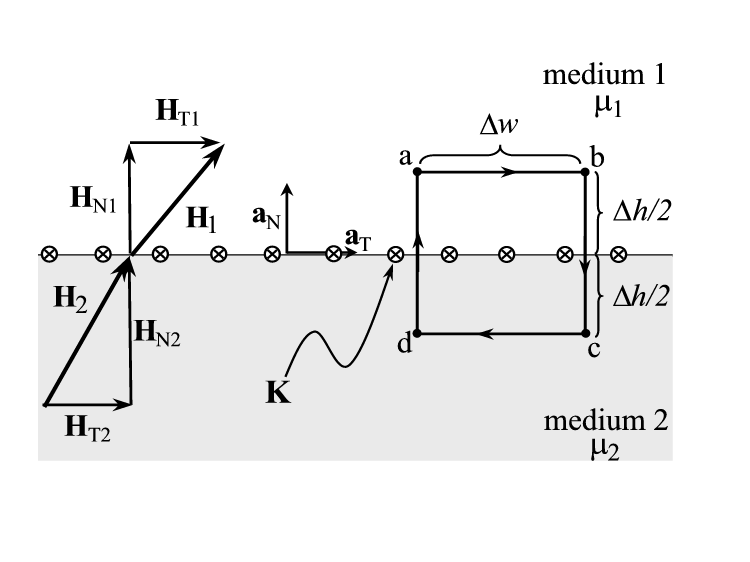
\includegraphics[width=0.5\linewidth]{./lect7/pic1.png}
\end{center}
Taking integral on small box on boudary we get
$$0 = \oint \div{\va{B}} \dd[3]{r} = \oint \va{B} \vdot \dd{s} = \qty(\va{B}_{1,\perp}-\va{B}_{2,\perp}) \Delta s$$
i.e. 
$$\va{B}_{1,\perp}=\va{B}_{2,\perp}$$

What happens with $B_\parallel$?

$$\oint \va{B}\vdot \dd{\va{l}} = \frac{4\pi}{c} \int \va{j} \vdot \dd{\va{s}} = I  = \frac{4\pi}{c} K \dd{l}$$
$$\qty(B_{2, \parallel} - B_{1, \parallel}) = \frac{4\pi}{c} \va{K}  \dd{l}$$
$$\vu{n} \cross (\va{B}_2 - \va{B}_1) = \frac{4\pi}{c} \va{K} $$
where $\va{K}$ is surface current density.
\paragraph{Magnetic scalar potential}
It's impossible to write $\va{B} = -\grad{\phi_m}$. However, if there is some area in which there is no current, we can try to do so, since $\curl{\va{B}} = 0$.
Using Biot-Savart law
$$\va{B}(\va{r})= \frac{I}{c} \oint \dd{\va{r'}} \cross \frac{\va{r}-\va{r'}}{\abs{\va{r}-\va{r'}}^3} = \frac{I}{c} \underbrace{\oint \dd{r'} \cross \underbrace{\va{U}(\va{r})}_{\frac{\va{r}-\va{r'}}{\abs{\va{r}-\va{r'}}^3}}}_{\va{H}}$$
For some constant vector $\va{k}$:
$$\va{k}\vdot \va{H} = \va{k} \vdot \oint \dd{\va{r'}} \cross \va{U}(\va{r}) = \oint \dd{\va{r'}} \vdot \qty(\va{U} \cross \va{k}  ) = \int \dd{\va{s}} \cdot \curl(\va{U} \cross \va{k}) = \int \dd{\va{s}} \cdot \qty[ (\va{k} \vdot \grad)\va{U} - \va{k} (\div{\va{U}})]$$

where
$$(\va{k} \vdot \grad)\va{U} = \sum_{\alpha, \beta } k_\alpha  \pdv{U_\beta}{x_\alpha} \vu{x}_\beta$$
We can rewrite as

$$(\va{k} \vdot \grad)\va{U} = \sum_{\alpha } \qty(k_\alpha \vu{x}_\alpha) \vdot \sum_{\alpha, \beta } \qty(\pdv{U_\beta}{x_\alpha} \vu{x}_\beta \vu{x}_\alpha)$$
Denote matrix of derivatives $\pdv{U_\beta}{x_\alpha} \vu{x}_\beta \vu{x}_\alpha$ as $\grad{\va{U}}$, i.e., dyadic or outer product of $\grad$ and $\va{U}$.
Then
$$\oint \dd{\va{r'}} \cross \va{U}(\va{r}) = \int \grad{\va{U}} \vdot \dd{\va{s}} - \int \dd{s} \div{\va{U}}$$
In our case $\va{U} =\frac{\va{r}-\va{r'}}{\abs{\va{r}-\va{r'}}^3}$ and since $\va{r} \neq \va{r'}$, $\div{\va{U}} = 0$.
Finally, we got
$$\va{B}(\va{r}) = \frac{I}{c} \int \grad_{r'}{\frac{\va{r}-\va{r'}}{\abs{\va{r}-\va{r'}}^3}} \vdot \dd{\va{s'}} = -\frac{I}{c} \int \grad_r{\frac{\va{r}-\va{r'}}{\abs{\va{r}-\va{r'}}^3}} \vdot \dd{\va{s'}} = -\frac{I}{c} \grad_r{\int \frac{\va{r}-\va{r'}}{\abs{\va{r}-\va{r'}}^3}} \vdot \dd{\va{s'}}$$
That means
$$\phi_m(\va{r}) = \frac{I}{c} \grad_r{\int \frac{\va{r}-\va{r'}}{\abs{\va{r}-\va{r'}}^3}} \vdot \dd{\va{s'}}$$
such that
$$\va{B}= -\grad \phi_m(\va{r})$$

\paragraph{Geometrical meaning of $\phi_m$}
Suppose $\va{r}=0$. Then

$$\phi_m(\va{r}) = \frac{I}{c} \grad_r{\int -\frac{\va{r'}}{{r'}^3}} \vdot \dd{\va{s'}}$$
Note that $\frac{\va{r'}\vdot \dd{\va{s'}}}{{r'}^3} $ is solid angle $\Omega$ of current loop, i.e.
$$\phi_m = \frac{I}{c} \Omega$$

\subsection{Multipole expansion of magnets}
First of all for $\va{E}$ monopole is sum of charges, however there is no such thing as magnetic monopole.
\paragraph{Exercise}
Suppose there exists magnetic monopole $\va{B}= \frac{Q_B \vu{r}}{r^2}$. Solve the problem of movement
$$m\ddot{r} = \va{F}_B = \frac{q}{c} \va{v} \cross \va{B}$$

Write down the scalar potential
$$\phi_m = \frac{I}{c} \int \dd{s'} \cdot \frac{\va{r} - \va{r'}}{\abs{\va{r} - \va{r'}}^3}$$
\paragraph{First order approximation}
$r' \approx 0$:
$$\phi_m \approx \frac{I}{c} \int  \dd{s'} \vdot \frac{\va{r}}{r^3} = \frac{I}{c} \frac{\va{r}}{r^3}  \vdot  \int  \dd{s'} = \va{M} \vdot \frac{\va{r}}{r^3}$$
where
$$\va{M}= \frac{I}{c} \va{S}$$
is magnetic moment.

Alternatively we could use vector potential:
$$\va{A} = \frac{1}{c} \int \dd[3]{r'} \frac{\va{j}(\va{r'})}{\abs{\va{r}-\va{r'}}}$$
Taking Taylor series of $\frac{1}{\abs{\va{r}-\va{r'}}}$ around 0, we get
$$\va{A} \approx \frac{1}{cr} \int \va{j}(\va{r'}) \dd[3]{r'} +  \frac{\va{r}}{cr^3} \vdot \int \va{r'} \va{j}(\va{r'}) \dd[3]{r'}$$
($\frac{1}{\abs{\va{r}-\va{r'}}} \approx \frac{1}{r} + \frac{\va{r}\vdot \va{r'}}{r^3}$, thus we have a matrix under integral).
Note since
$$\pdv{x'_\beta}{x'_\alpha} = \delta_{\alpha\beta}$$
is identity matrix, we can rewrite
$$\int \va{j} \dd[3]{r'} =\int j_\alpha \cdot \pdv{x'_\beta}{x'_\alpha} \vu{x}_\beta \dd[3]{r'} = \int \pdv{x'_\alpha}\qty(j_\alpha x'_\beta \vu{x}_\beta) - x'_\beta \vu{x}_\beta\underbrace{ \pdv{j_\alpha}{x'_\alpha}}_{\div{\va{j}} = 0}\dd[3]{r'}$$
In matrix form:
$$\int \va{j} \dd[3]{r'} =\int \va{j} \vdot \pdv{x'_\beta}{x'_\alpha} \dd[3]{r'} = \int \div(\va{j}\va{x'})  - \qty(\div{\va{j}} )\va{r'} \dd[3]{r'}$$
Now, since there are no currents
$$\int \pdv{x'_\alpha}\qty(j_\alpha x'_\beta \vu{x}_\beta) \dd[3]{r'} = \int \dd{s'_\alpha} j_\alpha x'_\beta \vu{x}_\beta = 0$$
$$ \int \div(\va{j}\va{x'})  =  \int \dd{s'_\alpha} \va{j}\va{x'}  = 0$$
Thus
$$\int \va{j} \dd[3]{r'} =0$$


Now for second-order part, take one element of it:
$$ \eval{\int \va{r'} \va{j}(\va{r'}) \dd[3]{r'}}_{\alpha} = \int j_\beta \vu{x}'_\beta x'_\alpha \dd[3]{r'} = \frac{1}{2} \int j_\beta x'_\beta  x'_\alpha \dd[3]{r'} + \frac{1}{2} \int x'_\beta \vu{x}'_\beta j_\alpha \dd[3]{r'} + \frac{1}{2} \int j_b \vu{x}'_\beta x'_\alpha \dd[3]{r} - \frac{1}{2} \int x'_\beta \vu{x}'_\beta j_\alpha \dd[3]{r} $$
$$\vu{x'}_\beta \pdv{x'_\gamma} \qty(x'_\alpha x'_\beta j_\gamma ) = j_\alpha x'_\beta \vu{x'}_\beta + j_\beta x'_\alpha \vu{x'}_\beta + x'_\alpha x'_\beta \vu{x'}_\beta \underbrace{\pdv{j_\gamma}{x'_\gamma}}_{0} $$
$$\div{\va{j}\va{r}\va{r}} = \va{r}\va{j}\cdot \grad{\va{r}}) + (\va{j}\cdot \grad{\va{r}})\va{r} + \underbrace{\div{\va{j}}\va{r}}_{0}$$
Thus
$$ \frac{1}{2} \int j_\beta \vu{x'}_\beta  x'_\alpha \dd[3]{r'} + \frac{1}{2} \int x'_\beta \vu{x}'_\beta j_\alpha \dd[3]{r'} =\frac{1}{2} \int \vu{x'}_\beta \pdv{x'_\gamma} \qty(x'_\alpha x'_\beta j_\gamma )  \dd[3]{r'} =  \frac{\vu{x'}_\beta}{2} \oint  x'_\alpha x'_\beta \va{j} \vdot \dd{\va{s}}$$
$$ frac{1}{2}\int \va{r'} \va{j}\qty(\va{r'}) -\va{j}\qty(\va{r'})\va{r'}  \dd[3]{r'} = frac{1}{2}\int \div{\va{j}\va{r}\va{r}} \dd[3]{r'} = frac{1}{2} \oint \va{j}\va{r}\va{r} \dd[3]{r'}$$
If there are no currents inside, the integral is 0.

From second part we can acquire (from bac-cab identity):
$$A_2  = \frac{1}{2cr^3} \int \va{r} \vdot \qty[\va{r'} \va{j}\qty(\va{r'}) +\va{j}\qty(\va{r'})\va{r'}  ]\dd[3]{r'} = \qty[\frac{1}{2c} \int \va{r'} \cross \va{j}\qty(\va{r'}) \dd[3]{r'} ] \cross \frac{\va{r'}}{r^3} = \va{M} \cross \frac{\va{r}}{r^3}$$ 

If the loop is in plane,  $\int \va{r'} \cross \dd[3]{r'}$ is area and thus
$$\va{M} = \frac{I}{2c} \int \va{r'} \cross \dd[3]{r'} = \frac{I}{2c} \va{S}$$

\paragraph{Connection with angular momentum}
$$\va{j} = \rho_e \va{v}_e$$
Substituting
$$\va{M} = \frac{1}{2v} \int \va{r} \cross \rho_e \va{v}_e \dd[3]{r}$$
This looks pretty much like angular momentum
$$\va{L} =  \int \va{r} \cross \rho_m \va{v}_m \dd[3]{r}$$
If $\rho_m \propto \rho_e$ and $v_m \propto v_e$ (e.g., there is one kind of current carriers), $\va{L}\propto \va{M}$. For $v_e=v_m$, we get
$$\va{M} = \frac{q}{2mc} \va{L}$$
We define gyromagnetic relation $\frac{M}{L}$.
\paragraph{Bohr magneton} $$M_B = \frac{e\hbar}{2mc}$$
\paragraph{Electromagnetic force}
$$\va{F} = q\va{E}  + q\frac{\va{v}}{c}\cross \va{B}$$
If $\va{E} = 0$, power of force
$$\va{F} \vdot \va{B} = \qty(q\frac{\va{v}}{c}\cross \va{B}) \vdot \va{v}= 0$$

So for magnetic force:
$$\dd{\va{F}} = \frac{1}{c} \sum_{\alpha \in \dd{l}} q_\alpha \va{v}_\alpha \cross \va{B} = \frac{I}{c} \dd{\va{l}} \cross \va{B}$$

Suppose we have long wire with $\va{I} = I\vu{x}$ and external field $\va{B} = B\va{y}$. If ve move wire in direction $-\vu{z}$, we need to spend energy, however magnetic field doesn't apply work. Where the energy goes? Since now particles have velocity in direction $\vu{z}$, the field accelerates them.

\paragraph{Energy of $\va{B}$}
In case of electric field we got energy $\frac{E^2}{8\pi}$. Unsuprisingly for magnetic field we get $\frac{B^2}{8\pi}$.

Suppose we have infinite plane of current $\dd{I} = K \dd{l}$ and one parallel plane with current in opposite direction.

What is work per unit area required to move the plane by distance $h$?

Now since the field $B_0$ is constant inside and 0 outside, the work is exactly the energy of the magnetic field.

What is the field of the lower plane?
$$\curl{\va{B}} = \frac{4\pi}{c} \va{j}$$
$$\int \curl{\va{B}} \vdot \dd{\va{s}} = \oint \va{B} \vdot \dd{l}$$
$$\frac{4\pi}{c} KL_0 = 2BL_0$$
Thus
$$B = \frac{2\pi}{c} K$$

Since force is $\dd{\va{F}} =\frac{I}{c} \dd{\va{l}_I} \cross \va{B}$
where $\va{l}_I$ is direction of current. Then force on upper plane is
$$\dd{F} = \frac{I}{c}\dd{l_0}  = \frac{K}{c}\dd{l}\dd{l_0} B $$
And thus the work is
$$\dd{W} = \underbrace{h\dd{l}\dd{l_0}}_{\text{volume element}} \frac{K}{c}B = \dd{V} \frac{B^2}{2\pi} =  \dd{V} \frac{B^2_0}{8\pi}  $$
i.e., the energy per volume is $\frac{B^2}{8\pi}$.

\paragraph{Energy of magnetic dipole moment in external magnetic field}

\paragraph{Force of $\va{B}$ on system of currents}
$$\va{F}= \frac{q}{c} \va{v} \cross \va{B}$$
(for comparison, Coriolis force is $\va{F} = -2 \va{\Omega} \cross \va{v}$).

Then
$$\dd{\va{F}} = \frac{I}{c}\dd{l} \cross \va{B}$$
i.e.,
$$\va{F} = \frac{I}{c}\oint \dd{l} \cross \va{B} $$
Taylor series of $\va{B}$ is
$$\va{B} \approx \va{B}(0) + \eval{(\va{r} \vdot \grad)\va{B}}_{\va{r}=0}$$
Thus 
$$\va{F} = \frac{I}{c} \oint \dd{\va{r}} \cross \qty[\va{B}(0) + \eval{(\va{r} \vdot \grad)\va{B}}_{\va{r}=0}] = \frac{I}{c} \oint \dd{\va{r}} $$
Since
$$\oint \dd{\va{r}} \cross \va{u}= \int (\grad \va{u}) \vdot \dd{\va{s}} - \int \dd{\va{s}} (\div{\va{u}}) $$
we get
$$\va{F} = \frac{I}{c} \int \grad((\va{r} \vdot \grad)\va{B})\vdot \dd{s} = \frac{I}{c} \int \dd{s} \div[(\va{r} \vdot \grad)\va{B}] = \frac{I}{c} \int \dd{s} \div{\va{B}} = 0$$
In case of magnetic dipole:
\begin{align*}
\va{F} = \frac{I}{c} \int  \grad(\va{r} \vdot\qty(  \grad\va{B})_{r=0})\vdot \dd{s} = \frac{I}{c} \int  \grad(x_\alpha \vdot\qty(  \partial_\alpha \va{B})_{r=0})\vdot \dd{s}
= \frac{I}{c} \int  \vu{x}_\beta \partial_\beta\qty(x_\alpha \vdot\qty(  \partial_\alpha B_\gamma \vu{x}_\gamma )_{r=0})\vdot \dd{s_\delta \vu{x}_\delta} 
=\\= \frac{I}{c} \int  \vu{x}_\beta \delta_{\alpha\beta} \qty( \partial_\alpha B_\gamma \vu{x}_\gamma )_{r=0}\vdot \dd{s_\delta \vu{x}_\delta} 
= \frac{I}{c} \int  \vu{x}_\alpha \qty( \partial_\alpha B_\gamma  )_{r=0}\vu{x}_\gamma\vdot \dd{s_\delta \vu{x}_\delta} 
= \frac{I}{c} \int  \vu{x}_\alpha \qty( \partial_\alpha B_\gamma  )_{r=0} \dd{s_\gamma} 
=\\=  \vu{x}_\alpha \qty( \partial_\alpha B_\gamma  )_{r=0} \frac{I}{c} \int  \dd{s_\gamma} = \grad{B} \vdot \va{M}
= \grad(\va{M} \cdot \va{B})
\end{align*}
Then the energy of magnetic dipole moment in external magnetic field is
$$U = \va{M} \vdot \va{B}$$
\paragraph{Landau's method}
Looking at average in time:
$$F = \expval{\sum \frac{q}{c}\va{v}_\alpha \cross \va{B}} = \expval{\dv{t} \sum \frac{q}{c}\va{r}_\alpha \cross \va{B}} \to 0$$
Since if $X$ doesn't diverges
$$\dv{t} \bar{X} = \frac{1}{T} \int_0^T \dv{X}{t} \dd{t} = \frac{X(T)-X(0)}{T} $$

Now, the torque is
$$\va{N} = \expval{\sum \frac{q}{c} \va{r}_i \cross \qty(\va{v} \cross \va{B})} = \expval{\sum \frac{q}{c} \va{v} \qty(\va{r}\vdot \va{B}) - \va{B} \qty(\va{v} \vdot \va{r})}$$
Similarly, 
$$\va{v}\vdot \va{r} = \dv{r^2}{t}$$
on average gives $0$, i.e.,
$$\va{N} = \expval{\sum \frac{q}{c} \va{v}(\va{r} \vdot \va{B})}$$
$$\va{v}(\va{r} \vdot \va{B}) = \underbrace{\frac{1}{2} \dv{t}\qty[\va{r}(\va{r} \vdot \va{B})]}_{0} + \underbrace{\frac{1}{2} \va{v}(\va{r} \vdot \va{B}) - \frac{1}{2} \va{r}(\va{v} \vdot \va{B})}_{\frac{1}{2} \va{v}\cross (\va{r} \cross \va{B})}$$
Define
$$\va{M} = \frac{1}{2c} \sum q\va{r} \cross \va{B}$$
Then
$$\va{N}  = \va{M} \cross \va{B} = \frac{1}{2c}\sum q\va{r} \cross \va{v}$$
\paragraph{Larmor precession}
The angular momentum vector $\va{M}$ precesses about the external field axis with an angular frequency known as the Larmor frequency,
$ \omega =-\gamma B$

where $\omega $ is the angular frequency, $\va{B}$ is the magnitude of the applied magnetic field. $\gamma$ is the gyromagnetic ratio of system.

\section{Electric field in insulating matter}
\paragraph{Exercise}
Suppose molecules are neutral conducting balls. What happens when appears external field? 
\paragraph{Field due to polarization}
Define polarization with vector $\va{P}$ and then electric dipole of volume $\Delta V$ is
$$\va{p} = \va{P} \Delta V $$ %TODO
$$\Phi_{dipole} = \frac{\va{P}\cdot \va{r}}{r^3}$$
$$\phi_{total} =- \int \dd[3]{r'} \frac{\va{r} - \va{r}'}{\abs{\va{r} -\va{r}'}}\vdot \va{P}(r) $$
$$ \va{E}_p = -\grad_r{\int \dd[3]{r'} \frac{\va{r}-\va{r}'}{\abs{\va{r}-\va{r}'}^3} \vdot \va{P}(\va{r}')}$$
$$\va{E}_p = -\int \dd[3]{r'}  \va{P}(\va{r}') \vdot \grad_r\frac{\va{r}-\va{r}'}{\abs{\va{r}-\va{r}'}^3}  = \int \dd[3]{r'}  \va{P}(\va{r}') \vdot \grad_{r'}\frac{\va{r}-\va{r}'}{\abs{\va{r}-\va{r}'}^3} = -\int \dd[3]{r'}  \frac{\va{r}-\va{r}'}{\abs{\va{r}-\va{r}'}^3}  \grad_{r'} \vdot \va{P}(\va{r}') + \oint \dd{\va{s}}  \vdot \va{P} (\va{r}') \frac{\va{r}-\va{r}'}{\abs{\va{r}-\va{r}'}^3}  $$
Here $\rho_b(\va{r}) = -\div{\va{P}}$ is induced charge density inside the matter.
$$\va{E}_p = \int \dd[3]{r'}  \frac{\va{r}-\va{r}'}{\abs{\va{r}-\va{r}'}^3} \rho_b(\va{r}) + \oint \dd{s'}  \sigma_b (\va{r}') \frac{\va{r}-\va{r}'}{\abs{\va{r}-\va{r}'}^3}  $$
where $\sigma_b = \vu{n} \vdot \va{P}$.

The total field thus is
$$\va{E} = \va{E}_{free} + \va{E}_p = \int \dd[3]{r'}  \frac{\va{r}-\va{r}'}{\abs{\va{r}-\va{r}'}^3} \qty(\rho_{free}(\va{r}) - \div{\va{P}}) + \oint \dd{s'}  \frac{\va{r}-\va{r}'}{\abs{\va{r}-\va{r}'}^3} \qty(\sigma_{free} + \vu{n} \vdot \va{P})$$

\subsection{Equations for field in matter}
$$\div{\va{E}} = 4\pi \rho_{free} - 4\pi \grad{\va{P}}$$
$$\vu{n}\vdot \qty(\va{E}_2-\va{E}_1) = 4\pi \qty[\sigma_{free} + \vu{n}(\va{P}_1-\va{P}_2) ]$$
We define electic displacement $\va{D}$:
$$\va{D} = \va{E} + 4\pi \va{P} \Rightarrow \div{\va{D}} = 4\pi \rho_{free}$$
$$\vu{n} \vdot (\va{D}_2 - \va{D}_1) = 4\pi \sigma_{free}$$

\paragraph{Connection between $\va{P}$, $\va{E}$, $\va{D}$}
Define susceptibility $\chi_E$
$$\va{P} = \chi_E\va{E} \Rightarrow \va{E} + 4\pi \va{P} = \epsilon \va{E}$$
when $\epsilon = 1+4\pi \chi_E$.

Note that in general case, $\va{D} = \epsilon \va{E}$, where $\epsilon$ is matrix which also might depend on $\va{r}$.

Thus our equations are:
$$\begin{cases}
\grad{\va{D}} = 4\pi \rho\\
\curl{\va{E}} = 0\\
E_{t,1}=E_{t,2}
\end{cases}$$

\paragraph{Uniqueness of solution}
Suppose there are two solutions, $\va{D}_1$ and $\va{D}_2$, define $\va{D} = \va{D}_1-\va{D}_2$.
$$\int \va{D}\vdot \va{E} \dd[3]{r} = -\int \va{D} \vdot \grad{\phi} \dd[3]{r} = - \int \qty[ \div(\phi\va{D}) - \phi \div{\va{D}}] \dd[3]{r}$$
Now
$$\va{D} \vdot \va{E} = \va{E} \epsilon \va{E}$$
if $\epsilon$ is scalar, $\va{D} \vdot \va{E} = \epsilon E^2$.

Since $\div{\va{D}} = 0$, we get
$$\int \va{D}\vdot \va{E} \dd[3]{r} = -\int \div(\phi\va{D}) \dd[3]{r} =-\oint \va{\phi} \va{D} \vdot \dd{\va{s}}$$

If $\va{D} \vdot \vu{n} = 0 $ or $\phi=0$ on the boundary, we get $\int \va{D}\vdot \va{E} \dd[3]{r} = 0$. Now if $\epsilon$ is positive (or positive defined in case of matrix), we conclude that $\va{E}=0$. This provides us with two kinds of boundary conditions - $\va{D} \vdot \vu{n} $ or $\phi$ should be given on boundary.

\paragraph{Force on test charge}
Note that force on test charge in dielectric matter is $\va{E}q$.
\paragraph{Example}
Suppose we have matter with $\epsilon>1$ inside other matter with $\epsilon=1$. Also there is point charge inside first one (located in origin).Then
$$\va{D}= \frac{q}{r^2}\vu{r}$$
$$\va{E} = \frac{\va{D}}{r^2}\vu{r}= \frac{q}{\epsilon r^2}\vu{r}$$
However
$$\va{p} = \frac{\va{D} - \va{E}}{4\pi}$$
and outside of origin
$$\div{\va{p}} = 0$$
\paragraph{Surface charge}
There is discontinuity in normal part of $\va{E}$ and similarly there is discontinuity in normal part of $\va{D}$
\paragraph{$\epsilon$ of conductor}
Since in conductor there is no field, we an choose $\epsilon=\infty$ 
\paragraph{Example}
Suppose we have dieletric matter in $x>0$ and a charge $q$ in $x=-d$ in vacuum.

First of all, $\rho_d = 0$, since there is charges inside of dielectric. Thus the only source of field is $\sigma_b$.
$$\sigma_b = \vu{n} \vdot \va{P} = \vu{n} \vdot \qty(\chi_E \va{E}) = \chi_E \vu{n} \vdot \va{E}$$
$$\va{E} = \va{E}_q + \va{E}_{\sigma_b}$$
$$\va{E}_q \vdot \vu{n}= -\frac{qd}{(R^2+d^2)^{\frac{3}{2}}}$$
$$\vu{n} \vdot \va{E}_{\sigma_b} = -2\pi \sigma_b$$
$$\sigma_b = \chi_E \qty[ -\frac{qd}{(R^2+d^2)^{\frac{3}{2}}} -  2\pi \sigma_b ]$$
Thus
$$\sigma_b = -\frac{\chi_E}{1+2\pi \chi_E} \frac{qd}{(R^2+d^2)^{\frac{3}{2}}} $$
and
$$q_b = \int \sigma_b \dd{s} = -\frac{2\pi \chi_e}{1+2\pi \chi_e} q$$
And thus in limit $\chi_e \to \infty $ we get $q_b \to -q$.

\subsection{Magnetic field in matter}
Describe molecules as magnetic dipole. Then their dipole moment $\va{\mu}$ will try to turn into direction $\va{B}$:
$$\va{\mu} = \va{M}(\va{r}) \Delta V$$
Then
$$\va{A}_n = \int \dd[3]{r'}\va{M}(\va{r}) \cross \frac{\va{r}-\va{r}'}{\abs{\va{r}-\va{r}'}^3} = \int \dd[3]{r'}\va{M}(\va{r}) \cross \grad_{r'} \frac{1}{\abs{\va{r}-\va{r}'}} = \oint \frac{\va{M}(\va{r}') \cross \dd{\va{r}'}}{\abs{\va{r}-\va{r}'}} + \int \frac{\grad_{r'}\cross \va{M}(\va{r}')}{\abs{\va{r}-\va{r}'}} \dd[3]{r'}$$
And total potential is
$$\va{A}_{tot} = \va{A}_{free} + \va{A}_{m} = \frac{1}{c} \int \dd[3]{r'} \frac{\va{j}(\va{r}') + c \curl{\va{M}(\va{r}')}}{\abs{\va{r}-\va{r}'}} + \frac{1}{c} \int \frac{\va{K}(\va{r}')\dd{s'} + c\va{M}(\va{r}') \cross \dd{\va{s}'}}{\abs{\va{r}-\va{r}'}}$$
We denote
$$\va{j}_b = c \curl{\va{M}}$$
and
$$\va{K}_b = c\va{M} \cross \vu{n}$$
\paragraph{Equations of magnetic field in matter}
$$\curl{\va{B}} = \frac{4\pi}{c} \qty(\va{j} + c\curl{\va{M}})$$
Define
$$\va{H} = \va{B} - 4\pi \va{M}$$
And thus
$$\curl{\va{H}} = \frac{4\pi}{c} \va{j}$$
We define $\chi_M$ as
$$\va{M}(\va{r}) = \chi_m \va{H}$$
and
$$\va{B}= (1+4\pi \chi_M) \va{H} = \mu \va{H}$$
$\mu$ is called permeability.

\section{Time-dependent $\va{E}$ and $\va{B}$ }
\paragraph{Faraday's law of induction}
$\va{B}(t)$ induces current in closed circuit.
Define $\Phi$, flux of magnetic field
$$\Phi = \int \va{B} \vdot \dd{\va{s}}$$
then EMF, $\mathcal{E}$ is
$$\mathcal{E} = \oint \va{E} \vdot \dd{\va{r}} = -\frac{1}{c} \dv{\Phi}{t} =-\frac{1}{c} \dv{t} \int \pdv{\va{B}}{t} \vdot \dd{\va{s}}$$
\paragraph{Lenz's law}
The direction of current induced in a conductor by a changing magnetic field due to induction is such that it creates a magnetic field that opposes the change that produced it.
\paragraph{Different description of Faraday's law}
Suppose we have $\va{B}(\va{r})$ independent on time. For some loop of current
$$\va{F} = \frac{q}{c} \va{v} \cross \va{B}$$
Integral on force on charge over the loop
$$\oint \frac{q}{c} (\va{v} \cross \va{B}) \vdot \dd{\va{r}}$$
And thus
$$\va{E} = \frac{\va{v}}{c} \cross \va{B}_{lab}$$
Then EMF is
\begin{align*}
\mathcal{E} = \oint \frac{1}{c} (\va{v} \cross \va{B}) \vdot \dd{\va{r}} = \frac{1}{c} \int \curl(\va{v} \cross \va{B}) \vdot \dd{\va{s}} = \frac{1}{c} \int \qty[\va{v}\qty(\div{\va{B}}) - (v \vdot \grad)\va{B} ] \vdot \dd{\va{s}} =\\= -\frac{1}{c} \int \qty(\va{v} \vdot \grad) \va{B} \vdot \dd{\va{s}} = -\frac{1}{c} \int \dv{\va{B}}{t} \vdot \dd{\va{s}} = -\frac{1}{c} \dv{t} \int \va{B} \vdot \dd{\va{s}}
\end{align*}
\paragraph{Full derivative}
$$\dv{F(\va{r}, t)}{t} = \lim_{\Delta t \to 0} \frac{F(\va{r}\qty\big(t+ \Delta t), t+\Delta t) - F\qty\big(\va{r}(t), t)}{\Delta t} = \pdv{F}{t} + \qty(\va{v} \vdot \grad) F$$

\paragraph{Example}
$$\va{B}= \va{B}(\va{r}, t)$$
$$\int\limits_{S_0} \curl{\va{E}} \vdot \dd{\va{s}}=\oint \va{E} \vdot \dd{\va{r}} = -\frac{1}{c} \int\limits_{S_0} \pdv{\va{B}}{t} \vdot \dd{\va{s}}$$
Since this is independent on $S_0$, we get
$$ \curl{\va{E}} = -\frac{1}{c} \pdv{\va{B}}{t}$$
which is one of Maxwell's equations:
\paragraph{Maxwell's equations}
$$\begin{cases}
\div{\va{D}} = 4\pi \rho\\
\curl{E} = -\frac{1}{c} \pdv{\va{B}}{t} \\
\div{\va{B}} = 0\\
\curl{\va{H}} = \frac{4\pi}{c} \va{j} + \frac{1}{c}\pdv{\va{D}}{t}
\end{cases}$$
$ \frac{1}{c}\pdv{\va{D}}{t}$ is called displacement current, we can see that it's needed from $\div{\curl{H}} = 0$:
$$\pdv{\rho}{t} + \div{\va{j}} = 0$$

If there were magnetic monopoles we would have, in vacuum:
$$\begin{cases}
	\div{\va{E}} = 4\pi \rho\\
	\curl{E} = -\frac{1}{c} \pdv{\va{B}}{t} \textcolor{red}{-\frac{4\pi}{c}\va{j}_m} \\
	\div{\va{B}} = 0\textcolor{red}{+4\pi \rho_m}\\
	\curl{\va{B}} = \frac{4\pi}{c} \va{j} + \frac{1}{c}\pdv{\va{D}}{t}
\end{cases}$$
i.e., equations are fully symmetric.
\paragraph{Duality transformation}
If we define 
$$\begin{pmatrix}
\rho_e\\\rho_m
\end{pmatrix} = \begin{pmatrix}
\cos \psi&-\sin \psi\\\sin \psi&\cos \psi
\end{pmatrix}\begin{pmatrix}
\rho_e'\\\rho_m'
\end{pmatrix}$$
$$\begin{pmatrix}
\va{E}\\\va{B}
\end{pmatrix} = \begin{pmatrix}
\cos \psi&-\sin \psi\\\sin \psi&\cos \psi
\end{pmatrix}\begin{pmatrix}
\va{E}'\\\va{B}'
\end{pmatrix}$$
new quantities fulfill generalized Maxwell equations. If for all particles $\frac{q_m}{q_e} = \text{const}$, we can choose $\psi$ such that $\rho_m = 0$.

\section{Relativity}
\paragraph{Lorentz trasformation}
$$\begin{cases}
x = \frac{x'+v't}{\sqrt{1-\frac{v^2}{c^2}}}\\
t = \frac{t'+\frac{v}{c^2}x'}{\sqrt{1-\frac{v^2}{c^2}}}\\
y=y'\\
z=z'
\end{cases}$$
\paragraph{4-vector}
$x^0=ct$, $x^1=x$, $x^2=y$, $x^3=z$, this is contravariant 4-vector
$$x^i = \qty(ct, \va{r})$$
Covarient 4-vector is
$$x_i = \qty(ct,, -\va{r})$$
Einstein summation convention is
$$x_ix^i = \sum_{i=0}^3 = x_ix^i = (ct)^2 - r^2$$
\paragraph{Metric}
Define $g_{ij}$ such 
$$x_i = g_{ij} x_j$$
i.e.,
$$g = \begin{pmatrix}
1&0&0&0\\
0&-1&0&0\\
0&0&-1&0\\
0&0&0&-1
\end{pmatrix}$$
Denote $\eta=g$.
\paragraph{Examples of metrics}
In 3D, we have identity metric
$$\dd{r^2} = \dd{x^2} + \dd{y^2} + \dd{z^2}$$
However on sphere 
$$\dd{l^2} = \sin[2](\theta) \dd{\phi^2} +b\dd{\theta^2}$$
i.e. metric is not identity.
\paragraph{4-vector in electromagteics}
$$A^i = \qty(\phi, \va{A})$$
Denote $A^0 = \phi$.

Then
$$A_iA^i = {A^0}^2 + \va{A}^2$$

\paragraph{Transformation of 4-vector}
$$A^0 = \frac{{A^0}' + \frac{v}{c}{A^1}'}{\sqrt{1-\frac{v^2}{c^2}}}$$
$$A^1 = \frac{{A^1}' + \frac{v}{c}{A^0}'}{\sqrt{1-\frac{v^2}{c^2}}}$$

For covariant vector
$$\phi = \frac{{A^0}' - \frac{v}{c}{A^1}'}{\sqrt{1-\frac{v^2}{c^2}}}$$
$$A^1 = \frac{{A^1}' - \frac{v}{c}{A^0}'}{\sqrt{1-\frac{v^2}{c^2}}}$$

We can write in matrix form
$$A^i = L_j^i {A^j}'$$
\paragraph{Tensor}
Example of tensor wold be $A^iA^j$. To apply transform on tensor, we apply 
$$T^{lm} = L_{i}^l L_j^m {T'}^{ij}$$
\paragraph{Example}
$$\dd{s^2} = \dd{x_i} \dd{x^i} = c^2\dd{t^2} - (\dd{\va{r}})^2 = c^2\dd{t^2} \qty(1-\frac{\va{v}^2}{c^2}) \Rightarrow \dd{s} = \dd{t} \sqrt{1+\frac{v^2}{c^2}}$$
We define velocity
$$u^i = \dd{x^i}{s} = \qty(\frac{c\dd{t}}{c\dd{t}\sqrt{1-\frac{v^2}{c^2}}}, \frac{\dd{r}}{c\dd{t}\sqrt{1-\frac{v^2}{c^2}}}) = \qty(\frac{c\dd{t}}{c\dd{t}\sqrt{1-\frac{v^2}{c^2}}}, \frac{\dd{r}}{c\dd{t}\sqrt{1-\frac{v^2}{c^2}}}) = \qty(\frac{1}{\sqrt{1-\frac{v^2}{c^2}}}, \frac{\va{v}}{c\sqrt{1-\frac{v^2}{c^2}}})$$

Note that
$$u_iu^i = \dv{x^i}{s}\dv{x_i}{s} = \frac{\dd{x_i}\dd{x^i}}{\dd{s^2}}  = \frac{\dd{s^2}}{\dd{s^2}} = 1$$

Now define 4-vector of energy and momentum $p^i = mcu^i$. Then
$$p^y = \frac{m\dd{y}}{\dd{s}}$$
is conserved in all frames of reference.

\paragraph{Lagrangian of particle in electromagnetic field}
$$S =\int \mathcal{L}(t) \dd{t}$$
$$\mathcal{L}_{free} = -mc^2\sqrt{1-\frac{v^2}{c^2}}$$
Note that $\mathcal{L} \dd{t}$ is $\dd{s}$, which is invariant.

$$\mathcal{L} = -mc^2\sqrt{1-\frac{v^2}{c^2}} - q\phi +\frac{q}{c}\va{A} \vdot \va{v}$$

Then generalized momentum:
$$\va{P} = \pdv{\mathcal{L}}{\va{v}} =\underbrace{ \frac{m\va{v}}{\sqrt{1-\frac{v^2}{c^2}}}}_{\va{P}_0} + \frac{q}{c}\va{A}$$
And Hamiltonian, or energy
$$\mathcal{H}= \va{v} \pdv{\mathcal{L}}{\va{v}}  - \mathcal{L} =  \frac{mc^2}{\sqrt{1-\frac{v^2}{c^2}}} + q\phi$$

Then movement equations are
$$\dv{t} \pdv{\mathcal{L}}{\va{v}} - \pdv{\mathcal{L}}{\va{r}} = 0$$
$$\dv{t} \qty(\va{P}_0+\frac{q}{c}\va{A}) = \frac{q}{c} \grad(\va{A} \vdot \va{v}) - q\grad{\phi}$$
$$\dv{\va{A}}{t} = \pdv{\va{A}}{t} + (\va{v} \vdot \grad)\va{A}$$
$$\frac{q}{c}\grad(\va{A} \vdot \va{v}) = \frac{q}{c} \qty(\va{v} \vdot \grad) \va{V} + \frac{q}{c} v \cross \qty(\curl{\va{A}})$$
$$\dv{P_0}{t} = -\frac{q}{c} \pdv{\va{A}}{t} - q\grad{\phi} + \frac{q}{c} \grad(\va{A} \vdot \va{v})$$

Define
$$\va{B} = \curl{\va{A}}$$
and
$$\va{E} = -\frac{1}{c} \pdv{\va{A}}{t} - \grad{\phi}$$
in this case we get Faraday's law:
$$\curl{\va{E}} = -\frac{1}{c} \pdv{t} \va{B}$$
\paragraph{Relativity}
$$\int \mathcal{L} \dd{t} = \int \qty[-mc\dd{s} -\frac{q}{c} A_i \dd{x^i}]$$
$$A_i\dd{x^i} =A_0\dd{x^0} + \va{A} \vdot \dd{\va{r}} = c\phi \dd{t} - \va{A} \vdot \va{v}\dd{t} $$
$$\delta S = 0 \Rightarrow -\int \qty[-mc^2 \frac{\dd{x_i}\dd{\delta x^i}}{\dd{s}} + \frac{q}{c} A_i \dd{\delta x^i} + \frac{q}{c} \delta A_i \dd{x^i}] = 0$$
Now
$$\delta A_i = \pdv{A_i}{x^k}\delta x^k$$
After manipulations we get
$$\delta S = \int \qty[mc\dv{u_i}{s} - \frac{q}{c}\qty(\pdv{A_k}{x_i} - \pdv{A_i}{x^k})] \delta x^i \dd{s} = 0$$
Define
$$F_{ik} = \pdv{A_k}{x_i} - \pdv{A_i}{x^k} $$
and movement equation 
$$m\dv{u_i}{s} = \frac{q}{c} F_{ik} u^k$$
$$F = \begin{pmatrix}
0&E_x&E_y&E_z\\
-E_x&0&-B_z&B_y\\
-E_y&B_z&0&-B_x\\
-E_z&-B_y&-B_x&0
\end{pmatrix}$$
or, rather
$$F_{ik} = \qty(\va{E}, \va{B})$$
and contravarient
$$F^{ik} = \qty(-\va{E}, \va{B})$$
\paragraph{Example}
For $i=0$;
$$mc \dv{u^0}{s} = \frac{q}{c} F^{0k}u_k = \frac{q}{c} (-E_x)\frac{-v_x}{\sqrt{1-\frac{v^2}{c^2}}}+\frac{q}{c} (-E_y)\frac{-v_y}{\sqrt{1-\frac{v^2}{c^2}}}+\frac{q}{c} (-E_z)\frac{-v_z}{\sqrt{1-\frac{v^2}{c^2}}}$$
$$\dd{} \frac{mc^2}{\sqrt{1-\frac{v^2}{c^2}}} = q \va{E} \vdot \va{v}$$
% TODO
\paragraph{4-vector of energy and momentum}
$$P^i = \qty(\frac{mc}{\sqrt{1-\frac{v^2}{c^2}}} +\frac{q}{c}\phi, \va{P} + \frac{q}{c}\va{A})$$
$$A_{i}\eta^{ij} = A^j$$
$$A_i = \eta_{ij}A^j$$
\paragraph{Invariants of electromagnetic field}
In case of tensor
$$F_k^i = \eta_{kj}F^{ij}$$
$$F_{kl} = \eta_{li}\eta_{kj}F^{ij}$$
$$F_{ij}F^{ij} = B^2-E^2$$
and
$$\epsilon^{ijkl}F_{ij}F^{kl} = \va{E} \vdot \va{B}$$
are invariant, where $\epsilon^{iklm}$ is Levi-Civita tensor.

That means that if $\va{E} \perp \va{B}$ or $\abs{\va{E}} = \abs{\va{B}}$

Also if $\va{E} \vdot \va{B} = 0$ there exists frame of reference where one of them is zero (which one depends on $E^2-B^2$). If one of invariants is non-zero, there always exists frame of reference where they are parallel.

$$\epsilon^{ijkl}F_{ij}F_{kl} = 4 \pdv{x^i} \qty(\epsilon^{ijkl}A_k \pdv{x_l} A_m)$$
which is $4D$ divergence. 

\paragraph{Maxwell equations}
$$\dv{\va{P}}{t} = q\va{E} + \frac{q}{c} \va{v} \cross \va{B}$$
where
$$\va{E} = -\grad{\phi} - \frac{1}{c} \pdv{\va{A}}{t}$$ 
and
$$\va{B} = \curl{\va{A}}$$
Thus
$$\curl{E} = -\frac{1}{c} \pdv{t} \curl{\va{A}} = -\frac{1}{c} \pdv{\va{B}}{t}$$
and
$$\div{\va{B}} = \grad(\curl{A}) = 0$$
i.e., first pair of Maxwell equations is determined exclusively by movement equations and doesn't require fields at all.

For second pair of Maxwell equations lets look at $\mathcal{L}$ of $A^i$ itself:
$$S = S_m+S_{mf}+S_f$$
where $S_m$ is action of particles, $S_{mf}$ is action of particle-field interactions and $S_f$ is filed action.
$$S_m = \sum_{particles} mc \int_a^b \dd{s}$$
$$S_{mf} = -\sum \frac{q}{c} \int A_k \dd{x^k}$$
$$\sum q A_k \dd{x^k} = \rho \dd[3]{x} A_k \dv{x^k}{t} \dd{t} = \rho \dv{x^k}{t} A_k \dd[3]{x} \dd{t} = j^k A_k \dd[3]{x} \dd{t} = j^k A_k \frac{\dd{\Omega}}{c}$$
where $\dd{\Omega} = \dd[4]{x}$, i.e.
$$S_{mf} = -\frac{1}{c^2} \int j^k A_k \dd{\Omega}$$
\subsection{Noether's theorem: connection between gauge invariance and charge conservation}
% Landau Field theory paragraph 27 and around
Note that $A_i \to A_i - \pdv{f}{x^i}$ doesn't change the fields:
$$\begin{cases}
\va{E} = -\frac{1}{c} \pdv{\va{A}}{t} - \grad{\phi}\\
\va{B}= \curl{\va{A}}
\end{cases}$$
Substituting
$$\begin{cases}
\tilde{\phi} = \phi - \frac{1}{c}\pdv{f}{t}\\
\va{\tilde{A}} = \va{A} + \grad{f}
\end{cases}$$
$$\curl{\va{\tilde{A}}} =\curl(\va{A} + \grad{\phi}) = \curl{\va{A}}$$
$$-\frac{1}{c} \pdv{\va{\tilde{A}}}{t} - \grad{\tilde{\phi}} = -\frac{1}{c} \pdv{t} \qty(\va{A} + \grad{f}) - \grad(\phi - \frac{1}{c} \pdv{f}{t}) = -\frac{1}{c} \pdv{\va{A}}{t} - \grad{\phi}$$

$$\tilde{S}_{mf} = -\frac{1}{c^2} \int j^i \tilde{A}_i \dd{\Omega} = -\frac{1}{c^2}\int j^i A_i \dd{\Omega} - \frac{1}{c^2}\int j^i \pdv{f}{x^i} \dd{\Omega} = S_{mf} - \frac{1}{c^2} \int \qty[\pdv{x^i} (fj^i) - f\pdv{j^i}{x^i}] \dd{\Omega}$$
From Gauss, first term of is 0, and thus the second has to be 0 too, resulting in charge conservation (or the other way around, from charge conservation we get gauge invariance).
\paragraph{Action of field $S_f$}
\begin{enumerate}
	\item Superposition princples dictates quadratic form in fields $\va{B}$ and $\va{E}$
	\item Action depends on fields and not on potential
	\item $\mathcal{L}$ has to be scalar, i.e. invariant under Lorentz transformation.
\end{enumerate}
Thus the action has of form $a\int F_{ik}F^{ik} \dd{\Omega}$. Since $F_{ik}F^{ik}=2(B^2-E^2)$, and $\va{E}$ contains $\pdv{\va{A}}{t}$, $a$ is negative so that action has minimum.

Thus the total action is
$$S = -\sum_{\text{particles}} \int mc \dd{s} - \frac{1}{c^2}A_i j^i \dd{\Omega} - \frac{1}{16\pi c} \int F_{ik}F^{ik} \dd{\Omega}$$
% Landau paragraph 30
Equating functional differential of $S$ to $0$:
$$0 = \delta S = -\frac{1}{c} \int \qty[\frac{1}{c} j^i \delta A_i + \frac{1}{8\pi} F^{ik}F_{ik}] \dd{\Omega}$$

Substituting
$$\delta F_{ik} = \delta \qty[\pdv{A_n}{x^i} - \pdv{A_i}{x^k}] = \pdv{\delta A_k}{x^i}-\pdv{\delta A_i}{x^k}$$
and
$$F^{ik} \pdv{\delta A_k}{x^i} =F^{ki}  \pdv{\delta A_i}{x^k} = - F^{ik} c $$
we get
$$F^{ik} \delta F_{ik} = -2 F^{ik}\pdv{\delta A_i}{x^k}  $$
and thus
$$\delta S = -\frac{1}{c} \int \qty[\frac{1}{c} j^i \delta A_i - \frac{1}{4\pi} F^{ik}\pdv{\delta A_i}{x^k} ] \dd{\Omega}$$
and since
$$F^{ik}\pdv{\delta A_i}{x^k} = \pdv{\qty(F^{ik}\delta A_i)}{x^k} - \pdv{F^{ik}}{x^k} \delta A_i$$
applying Gauss law

$$\delta S = -\frac{1}{c} \int \qty(\frac{1}{c} j^i  + \frac{1}{\pi}\pdv{F^{ik}}{x^k})\delta A_i \dd{\Omega}- \frac{1}{4\pi c} \int F^{ik} \delta A_i \dd{S_k}$$
Since surface integral is zero, we get

$$\int \qty(\frac{1}{c} j^i  + \frac{1}{\pi}\pdv{F^{ik}}{x^k})\delta A_i \dd{\Omega} = 0$$
$$ \frac{1}{\pi}\pdv{F^{ik}}{x^k} = \frac{4\pi}{c} j^i  $$


For $i=0$:
$$\pdv{F^{01}}{x}+\pdv{F^{02}}{y}+\pdv{F^{03}}{z} = -\frac{4\pi }{c} j^0$$
Since $j^0 = c\rho$, we get
$$\div{\va{E}} = 4\pi \rho$$
For $i=1$:
$$\pdv{F^{12}}{y}+\pdv{F^{13}}{z}+\frac{1}{c}\pdv{F^{10}}{t} = -\frac{4\pi }{c} j^1$$
$$\pdv{B_z}{y} - \pdv{B_y}{z} - \frac{1}{c} \pdv{E_x}{t} = \frac{4\pi}{c} j_x$$
i.e.,
$$\curl{\va{B}} = \frac{4\pi}{c} \va{j} + \frac{1}{c} \pdv{\va{E}}{t}$$
\paragraph{Energy density and energy flux}
$$\begin{cases}
\curl{\va{E}} = - \frac{1}{c} \pdv{\va{B}}{t}\\
\curl{\va{B}} =  \frac{1}{c} \pdv{\va{B}}{t} + \frac{4\pi}{c} \va{j}\\
\div{\va{B}}=0\\
\div{\va{E}} = 4\pi \rho
\end{cases}$$
$$\frac{1}{c} \va{E} \vdot \pdv{\va{E}}{t} + \frac{1}{c} \va{B}\vdot \pdv{\va{B}}{t} = \va{E} \vdot \qty[\curl{\va{B}} - \frac{4\pi}{c} \va{j}] - \va{B} \vdot \div{\va{E}} $$
$$\frac{1}{2c} \pdv{t} \qty( E^2+B^2) = - \frac{4\pi}{c} \va{j} \vdot \va{E}  - \div(\va{E} \cross \va{B})$$
$$ \pdv{t} \frac{E^2+B^2}{8\pi} = - \va{j} \vdot \va{E}  - \div(\va{S})$$
where $\va{S} = \frac{c}{4\pi} \va{E} \cross \va{B}$ is Poynting vector.

Physical meaning is that by integrating over the whole space
$$\dv{t} \int \frac{E^2+B^2}{8\pi} \dd[3]{r}= - \int \va{j} \vdot \va{E}] \dd[3]{r} - \underbrace{\oint \va{S} \vdot \dd{\va{a}}}_{0 \text{ for bounds in } \infty}$$
$$ \int \va{j} \vdot \va{E}] \dd[3]{r} = \sum q \va{v} \vdot \va{E} = \sum \va{v} \vdot \qty(m \dv{\va{v}}{t}) = \dv{t} (\sum \frac{1}{2} m v^2)$$
i.e., denoting kinetic energy by $K$,
$$\dv{t} \qty[\frac{E^2+B^2}{8\pi}  + K] = 0$$
\subsection{Action of field $S_f$}
\begin{enumerate}
	\item Superposition princples dictates quadratic form in fields $\va{B}$ and $\va{E}$
	\item Action depends on fields and not on potential
	\item $\mathcal{L}$ has to be scalar, i.e. invariant under Lorentz transformation.
\end{enumerate}
Thus the action has of form $a\int F_{ik}F^{ik} \dd{\Omega}$ (second invariant is full derivative). Since $F_{ik}F^{ik}=2(B^2-E^2)$, and $\va{E}$ contains $\pdv{\va{A}}{t}$, $a$ is negative so that action has minimum.

Thus the total action is
$$S = -\sum_{\text{particles}} \int mc \dd{s} - \frac{1}{c^2}A_i j^i \dd{\Omega} - \frac{1}{16\pi c} \int F_{ik}F^{ik} \dd{\Omega}$$
% Landau paragraph 30
Equating functional differential of $S$ to $0$:
$$0 = \delta S = -\frac{1}{c} \int \qty[\frac{1}{c} j^i \delta A_i + \frac{1}{8\pi} F^{ik}\delta F_{ik}] \dd{\Omega}$$

Substituting
$$\delta F_{ik} = \delta \qty[\pdv{A_k}{x^i} - \pdv{A_i}{x^k}] = \pdv{\delta A_k}{x^i}-\pdv{\delta A_i}{x^k}$$
and
$$F^{ik} \pdv{\delta A_k}{x^i} =F^{ki}  \pdv{\delta A_i}{x^k} = - F^{ik} \pdv{\delta A_i}{x^k} $$
we get
$$F^{ik} \delta F_{ik} = -2 F^{ik}\pdv{\delta A_i}{x^k}  $$
and thus
$$\delta S = -\frac{1}{c} \int \qty[\frac{1}{c} j^i \delta A_i - \frac{1}{4\pi} F^{ik}\pdv{\delta A_i}{x^k} ] \dd{\Omega}$$
and since
$$F^{ik}\pdv{\delta A_i}{x^k} = \pdv{\qty(F^{ik}\delta A_i)}{x^k} - \pdv{F^{ik}}{x^k} \delta A_i$$
applying Gauss law

$$\delta S = -\frac{1}{c} \int \qty(\frac{1}{c} j^i  + \frac{1}{\pi}\pdv{F^{ik}}{x^k})\delta A_i \dd{\Omega}- \frac{1}{4\pi c} \int F^{ik} \delta A_i \dd{S_k}$$
Since surface integral is zero, we get

$$\int \qty(\frac{1}{c} j^i  + \frac{1}{\pi}\pdv{F^{ik}}{x^k})\delta A_i \dd{\Omega} = 0$$
$$ \frac{1}{\pi}\pdv{F^{ik}}{x^k} = \frac{4\pi}{c} j^i  $$


For $i=0$:
$$\pdv{F^{01}}{x}+\pdv{F^{02}}{y}+\pdv{F^{03}}{z} = \frac{4\pi }{c} j^0$$
Since $j^0 = c\rho$, we get
$$\div{\va{E}} = 4\pi \rho$$
For $i=1$:
$$\pdv{F^{12}}{y}+\pdv{F^{13}}{z}+\frac{1}{c}\pdv{F^{10}}{t} = -\frac{4\pi }{c} j^1$$
$$\pdv{B_z}{y} - \pdv{B_y}{z} - \frac{1}{c} \pdv{E_x}{t} = \frac{4\pi}{c} j_x$$
i.e.,
$$\curl{\va{B}} = \frac{4\pi}{c} \va{j} + \frac{1}{c} \pdv{\va{E}}{t}$$
\paragraph{\textcolor{red}{What if $a$ was positive?}}

$$\begin{cases}
\curl{\va{E}} = - \frac{1}{c} \pdv{\va{B}}{t}\\
\curl{\va{B}} =  -\frac{1}{c} \pdv{\va{B}}{t} + \frac{4\pi}{c} \va{j}\\
\div{\va{B}}=0\\
\div{\va{E}} = -4\pi \rho
\end{cases}$$
Same charges start to attract.

In addition, we get inversion of Lenz law, i.e. induced current increases the magnetic field and magnetic field diverges.
\paragraph{Energy density and energy flux}
$$\begin{cases}
\curl{\va{E}} = - \frac{1}{c} \pdv{\va{B}}{t}\\
\curl{\va{B}} =  \frac{1}{c} \pdv{\va{B}}{t} + \frac{4\pi}{c} \va{j}\\
\div{\va{B}}=0\\
\div{\va{E}} = 4\pi \rho
\end{cases}$$
$$\frac{1}{c} \va{E} \vdot \pdv{\va{E}}{t} + \frac{1}{c} \va{B}\vdot \pdv{\va{B}}{t} = \va{E} \vdot \qty[\curl{\va{B}} - \frac{4\pi}{c} \va{j}] - \va{B} \vdot \div{\va{E}} $$
$$\frac{1}{2c} \pdv{t} \qty( E^2+B^2) = - \frac{4\pi}{c} \va{j} \vdot \va{E}  - \div(\va{E} \cross \va{B})$$
$$ \pdv{t} \frac{E^2+B^2}{8\pi} = - \va{j} \vdot \va{E}  - \div(\va{S})$$
where $\va{S} = \frac{c}{4\pi} \va{E} \cross \va{B}$ is Poynting vector.

Physical meaning is that by integrating over the whole space
$$\dv{t} \int \frac{E^2+B^2}{8\pi} \dd[3]{r}= - \int \va{j} \vdot \va{E}] \dd[3]{r} - \underbrace{\oint \va{S} \vdot \dd{\va{a}}}_{0 \text{ for bounds in } \infty}$$
Since
$$m\dv{\va{v}}{t} = q\va{E} + \frac{q}{c} \va{v} \cross \va{B}$$
$$ \int \va{j} \vdot \va{E} \dd[3]{r} = \sum q \va{v} \vdot \va{E} = \sum \va{v} \vdot \qty(m \dv{\va{v}}{t}) = \dv{t} (\sum \frac{1}{2} m v^2)$$
i.e., denoting kinetic energy by $K$,
$$\dv{t} \qty[\frac{E^2+B^2}{8\pi}  + K] = 0$$

\paragraph{Exercise} Derive the same equations in relativistic.

\paragraph{Maxwell equations in matter}
$$\begin{cases}
\curl{\va{E}} = - \frac{1}{c} \pdv{\va{B}}{t}\\
\div{\va{B}}=0\\
\curl{\va{H}} =  \frac{1}{c} \pdv{\va{D}}{t} + \frac{4\pi}{c} \va{j}\\
\div{\va{D}} = 4\pi \rho
\end{cases}$$

Now
\begin{align*}
\curl{\va{B}} = \frac{4\pi}{c} \qty(\va{j}_f+\va{j}_b) +\frac{1}{c} \pdv{t} \qty(\va{D}-\va{P}) =\frac{4\pi}{c} \va{j}_f+\frac{4\pi}{c} \va{j}_b +\frac{1}{c} \pdv{\va{D}}{t} -\frac{4\pi}{c}\pdv{\va{P}}{t} 
\end{align*}
But
$$\va{j}_b = c \curl{\va{M}} + \pdv{\va{P}}{t} $$

\begin{align*}
\curl{\va{B}} =4\pi\curl{\va{M}} + \frac{4\pi}{c}\pdv{\va{P}}{t} +\frac{4\pi}{c} \va{j}_f +\frac{1}{c} \pdv{\va{D}}{t} -\frac{4\pi}{c}\pdv{\va{P}}{t} 
\end{align*}
i.e.,
$$\curl{\va{H}} = \frac{4\pi}{c}\va{j}_f + \frac{1}{c} \pdv{\va{D}}{t}$$
\paragraph{Maxwell stress tensor}
We want to calculate force on volume element by electromagnetic fields.
\begin{align*}
\va{F}_E = \int \dd[3]{r} \rho \va{E}  = \int \dd[3]{r} \qty(\rho_{free}+\rho_{bound}) \va{E} = \frac{1}{4\pi} \int \dd[3]{r} (\div{\va{E}}) \va{E} = \frac{1}{4\pi} \int \dd[3]{r} \div(\va{E}\va{E}) - (\va{E} \vdot \grad)\va{E} =\\= \frac{1}{4\pi} \int \dd[3]{r} \qty[\div(\va{E}\va{E}) - \frac{1}{2}\grad\va{E}^2 + \va{E} \cross \qty(\curl{\va{E}}) ] = \frac{1}{4\pi} \int \dd[3]{r} \qty[\div(\va{E}\va{E}) - \frac{1}{2}\grad\va{E}^2 - \frac{1}{c}\va{E} \cross \pdv{\va{B}}{t}]
\end{align*}
$$$$
$$\va{F}_B = \int \dd[3]{r} \va{j} \cross \va{B}  = \int \dd[3]{r} \qty(\va{j}_{free}+\va{j}_{bound}) \cross \va{B} = \frac{1}{4\pi} \dd[3]{r} \qty(\curl{\va{B}} -\frac{1}{c}\pdv{\va{E}}{t} ) \cross{\va{B}} = \frac{1}{4\pi} \int \dd[3]{r} \qty[\div(\va{B} \va{B}) - \frac{1}{2}\grad{\va{B}^2} -\frac{1}{c}\pdv{\va{E}}{t} \cross \va{B} ]$$

The total force is
$$\va{F} = \frac{1}{4\pi} \int \dd[3]{r} \qty[\div(\va{E}\va{E}+\va{B} \va{B}) - \frac{1}{2}\grad(\va{E}^2+\va{B}^2 )- \frac{1}{c} \pdv{t} \qty(\va{E} \cross \va{B})]$$

Thus
$$\va{F}_\alpha= \int \dd[3]{r} \qty[\pdv{T_{\alpha \beta}}{x_\beta} - \frac{1}{4\pi c}\pdv{\va{E} \cross \va{B}}{t} ]$$
$$\va{F}= \int \dd[3]{r} \qty[\div{T} - \frac{1}{4\pi c}\pdv{\va{E} \cross \va{B}}{t} ]$$
where
$$T_{\alpha\beta} = \qty[E_\alpha E_\beta + B_\alpha B_\beta - \frac{1}{2}\delta_{\alpha \beta} (E^2+B^2) ]$$
$$T_{EB} = \qty[\va{D}\va{E} + \va{B}\va{H} - \frac{1}{2}\delta (E^2+B^2) ]$$
$$T_{DEBH} = \qty[\va{D}\va{E} + \va{B}\va{H} - \frac{1}{2}\delta (E^2+B^2) ]$$

Note that $T_{EB}$ gives force on all the matter, while $T_{DEBH}$ gives the force on free charges and currents (only for linear and homogeneous materials though).

By Gauss
$$F_\alpha = \oint T_{\alpha \beta} \dd{s_\beta} - \frac{1}{c^2} \dv{t} \int \va{S} \dd[3]{r}$$

Note that
$$\va{F} = \dv{P_{matter}}{t}$$
$$\dv{t} \qty(P_{matter}+\frac{1}{c^2} \int \va{S} \dd[3]{r}) = \oint T \vdot \dd{\va{s}}$$

Thus we can interpret 
$$P_{em} = \frac{1}{c^2} \int \va{S} \dd[3]{r}$$
as momentum of electromagnetic field.
\paragraph{Example}
Calculate force needed to keep charges on spherical surfaces:
$$F_{\alpha} = \oint T_{\alpha \beta} \dd{s_\beta} = \frac{E^2}{8\pi} \dd{s}$$
$$F = \frac{16 \pi^2 \sigma^2}{8\pi} = 2\pi^2 \sigma^2 $$

\paragraph{What happens in matter?}
If we want to know the force on free particles only, we need to replace $\va{E}\vdot \va{E}$ with $\va{E}\vdot \va{D}$ and $\va{B}\vdot \va{B}$ with $\va{B}\vdot \va{H}$ and thus
$$\va{P}_{em} = \frac{1}{4\pi c} \int \va{D} \cross \va{B}$$
Note that
$$\va{S} = \frac{c}{4\pi} \va{E} \cross \va{H}$$

\paragraph{Third law of Newton}
Suppose there is charge $q_1$ moving with velocity $-v_1\vu{x}$ and $q_2$ moving with velocity $-v_2\vu{y}$. If charges are close enough, the magnetic field by particles are in $\pm \vu{z}$ direction, and thus force on $q_2$ is in $\vu{x}$ direction and on $q_1$ in $\vu{y}$ direction. Thus the third law is broken, i.e., field's momentum has to change.


\paragraph{Angular momentum}
$$\va{L}  = \frac{1}{4\pi c} \int \va{r} \cross \qty(\va{E} \cross \va{B})\dd[3]{r}$$
\section{Electromagnetic waves}
If there is no free charges and currents:
$$\begin{cases}
\curl{\va{E}} = - \frac{1}{c} \pdv{\va{B}}{t}\\
\div{\va{B}}=0\\
\curl{\va{H}} =  \frac{1}{c} \pdv{\va{D}}{t} \\
\div{\va{D}} =0
\end{cases}$$

Suppose $\va{D} = \epsilon \va{E}$ and $\va{B} = \mu \va{H}$ for constant $\epsilon$ and we get
$$\begin{cases}
\curl{\va{B}} =  \frac{\epsilon \mu}{c} \pdv{\va{E}}{t} \\
\div{\va{E}} =0
\end{cases}$$

$$\curl(\curl{\va{E}}) = \grad(\div{E}) - \laplacian{\va{E}} = -\frac{1}{c} \pdv{\curl{\va{B}}}{t} = \frac{\epsilon \mu}{c} \pdv[2]{\va{E}}{t}  $$
We get wave equation:$$\laplacian{\va{E}} = \qty(\frac{\epsilon \mu}{c^2}) \pdv[2]{\va{E}}{t}$$
And similarly,
$$\laplacian{\va{B}} = \qty(\frac{\epsilon \mu}{c^2}) \pdv[2]{\va{B}}{t}$$
\paragraph{Solution}
Guess solution
$$\va{E}(\va{r}, t) = \va{E}_0 e^{\va{k} \vdot \va{r} - \omega t}$$
We can choose axis such that $\va{k} - k \vu{x}$:
$$\laplacian{\va{E}} = \pdv[2]{x} \va{E}_0 e^{i(kx-\omega t)} = -k^2\va{E}_0 e^{i(kx-\omega t)}$$
$$\pdv[2]{\va{E}}{t} = -\omega^2 \va{E}_0 e^{i(kx-\omega t)}$$
Thus
$$-\qty(\frac{\epsilon \mu}{c^2})\omega^2 \va{E}_0 e^{i(kx-\omega t)} = -k^2\va{E}_0 e^{i(kx-\omega t)}$$
$k$ is wavenumber, and
$$k^2 = \omega^2 \qty(\frac{\epsilon \mu}{c^2})$$
The velocity of wave propagation is
$$c_\epsilon = \frac{c}{\sqrt{\epsilon \mu}}$$
Since
$$\grad{\va{E}} = 0 = \pdv{x}E_{0x}e^{-i(kx - \omega t)}$$
Thus
$$E_{0x} = 0$$
i.e., EM wave is perpendicular to wave propagation direction.
In vacuum
$$\Box \va{E} = 0$$

If we substitute into Maxwell equation:
$$ i\va{k} \cross \va{E}  = \curl{\va{E}} = \frac{i\omega }{c}  \va{B}$$
$$\va{B} = \sqrt{\epsilon \mu} \vu{k} \cross \va{E}$$
In vacuum $\abs{B} = \abs{E}$ 
\subsection{Energy of field}
$$U = \frac{1}{8\pi} \qty(\va{E} \vdot \va{D} + \va{B} \vdot \va{H}) = \frac{1}{8\pi} \qty(\epsilon\va{E}^2 + \frac{\va{B}^2}{\mu}) $$
Since $\va{B}] = \sqrt{\epsilon \mu} E$
$$U = \frac{\epsilon}{4\pi} \va{E} \vdot \va{E} $$
Since $\va{E}$ is complex
$$U = \frac{\epsilon}{4\pi} \qty(\frac{\va{E}+\va{E}^*}{2})^2$$
Alternatively
$$\expval{U} = \frac{\int_0^T U \dd{t}}{\tau} = \frac{\epsilon }{8\pi} E_0^2$$

And similarly,
$$\expval{\va{S}} = \frac{c}{4\pi} \expval{\va{E} \cross \va{H}} = \frac{c\vu{k}}{8\pi} \sqrt{\frac{\epsilon}{\mu}} E_0^2$$
\paragraph{Pressure of radiation}
The momentum of electromagnetic wave
$$\va{G} = \frac{1}{4\pi c} \va{D} \cross \va{B}$$
and
$$\expval{\va{G}} = \frac{\epsilon\vu{k}}{8\pi c} \sqrt{\epsilon \mu} E_0^2$$
note that in vacuum
$$\va{G} = \frac{\va{S}}{c^2}$$

\paragraph{Refraction of EM waves}

\begin{center}	
	\includesvg[eps,svgpath = lect18/,width=0.5\linewidth]{pic01} %rotate
\end{center}

$$\va{E}  = \va{E}_0 e^{i\qty(\va{k} \vdot \va{r} - \omega t)}$$
where
$$k = \sqrt{\frac{\epsilon \mu}{c^2}} \omega$$
Since $\div{\va{D}} = 0$:
$$\epsilon_2 \vu{n}  \va{E}_2 e^{i\qty(\va{k}_2 \vdot \va{r} - \omega t)} = \epsilon_1 \vu{n} \qty(\va{E}_1 e^{i\qty(\va{k}_1 \vdot \va{r} - \omega t)}+\va{E}'_1 e^{i\qty(\va{k}'_1 \vdot \va{r} - \omega t)})$$
From $\curl{\va{E}} = -\frac{1}{c}\pdv{\va{B}}{t}$:
$$\vu{n} \cross \va{E}_2 = \vu{n} \cross \qty( \va{E}_1 e^{i\va{k}_1 \vdot \va{r}}+ \va{E}'_1 e^{i\va{k}'_1 \vdot \va{r}})$$
Similarly from other two Maxwell laws:
$$\epsilon_2 \vu{n}  \va{B}_2 e^{i\qty\va{k}_2 \vdot \va{r}} = \epsilon_1 \vu{n} \qty(\va{B}_1 e^{i\va{k}_1 \vdot \va{r} }+\va{B}'_1 e^{i\va{k}'_1 \vdot \va{r}})$$
$$\vu{n} \cross \va{B}_2 = \vu{n} \cross \qty( \va{B}_1 e^{i\va{k}_1 \vdot \va{r}}+ \va{B}'_1 e^{i\va{k}'_1 \vdot \va{r}})$$

Since the equations are fulfilled for any $\va{r}$ we get
$$\va{k}_1 \vdot \va{r} =\va{k}'_1 \vdot \va{r}=\va{k}_2 \vdot \va{r} $$

$$k_1' \sin(\theta'_1) = k_1 \sin (\theta_1) = k_2 \sin(\theta_2)$$
Since $\abs{k_1} = \abs{k'_1}$ we get
$$\theta_1 = \theta'_1$$

And we get Snell's law:
$$k_1 \sin(\theta_1) = k_2 \sin(\theta_2)$$
$$n_1 \sin(\theta_1) = n_2 \sin(\theta_2)$$
, where $n=\sqrt{\epsilon \mu}$.
\paragraph{Fermat's principle}
Fermat's principle or the principle of least time, is the principle that the path taken between two points by a ray of light is the path that can be traversed in the least time. 

Thus we can make optimization of 
$$d(y)= \frac{\abs{Ay}}{\frac{c}{n_1}}+\frac{\abs{yB}}{\frac{c}{n_2}}$$
and acquire Snell's law too.

\paragraph{Specific polarization}
Suppose $\va{E}_1$ parallel to plane of division, we get
$$\va{E}_1+\va{E}'_1 = \va{E}_2$$
$$\sqrt{\epsilon_1 \mu_1} (\va{E}_1 + \va{E}'_1) \sin(\theta_1) = \sqrt{\epsilon_1 \mu_1} \va{E}_2 \sin(\theta_2)$$
Assume $\mu=1$, we get
$$\begin{cases}
\va{E}_2 = \frac{2n_1 \cos(\theta_1)}{n_1 \cos(\theta_1) + n_2 \cos(\theta_2)}\va{E}_1\\
\va{E}'_1 = \frac{n_1 \cos(\theta_1) - n_2 \cos(\theta_2)}{n_1 \cos(\theta_1) + n_2 \cos(\theta_2)}\va{E}_1
\end{cases}$$
\paragraph{Electromagnetic waves in (non-ideal) conductor}
Define $\sigma$, conductance as
$$\va{j} = \va{E} \sigma$$
In this case
$$\curl{\va{B}} = \frac{4\pi}{c} \mu \sigma \va{E} + \frac{\mu \epsilon}{c}\pdv{\va{E}}{t}$$
If $\va{E},\va{B} \propto e^{i(\va{k}\vdot \va{r} - \omega t)}$ we get
$$i\va{k} \cross \va{B} = \frac{4\pi}{c} \mu \sigma \va{E} + \frac{i\omega \mu \epsilon}{c}\va{E}$$
and
$$i\va{k} \cross \va{E} = \frac{i\omega}{c} \va{B}$$
Multiplying by $\va{k}$
$$\frac{i}{\omega} (\va{k} \cross \qty(\va{k} \cross \va{E})) = -\frac{c\va{k}^2}{\omega} \va{E} = -\frac{\mu \epsilon \omega}{c} \qty(1+\frac{i4\pi \sigma}{\epsilon \omega})\va{E}$$
Thus we get dispersion relation
$$k = k_0\sqrt{1+\frac{i4\pi \sigma}{\epsilon \omega}}$$
where $k_0 = \frac{\sqrt{\epsilon \mu}}{c}\omega$.

Suppose $\va{k} = (\beta+i\abs{\alpha})\vu{x}$. We get
$$e^{i \va{k}\vdot \va{r}} = e^{i\beta x - \alpha x}$$
i.e.,
$$E,B \propto e^{-\alpha x}$$
\section{Fields of moving charges}
\paragraph{Radiation of electromagnetic waves}
$$\begin{cases}
\curl{\va{E}} = - \frac{1}{c} \pdv{\va{B}}{t}\\
\va{B}=\curl{\va{A}}\\
\curl{\va{B}} =  \frac{1}{c} \pdv{\va{E}}{t} + \frac{4\pi}{c} \va{j}\\
\div{\va{E}} = 4\pi \rho
\end{cases}$$
Substitute first pair into third equation:
$$\curl{\curl{\va{A}}} = \frac{1}{c} \qty[-\grad{\pdv{\Phi}{t}} - \frac{1}{c} \pdv[2]{\va{A}}{t}] + \frac{4\pi}{c} \va{j}$$
$$-\laplacian{\va{A}} + \grad(\div{\va{A}}) + \div(\frac{1}{c} \pdv{\Phi}{t}) = -\frac{1}{c^2} \pdv[2]{\va{A}}{t} + \frac{4\pi}{c}$$

We choose Lorenz gauge:
$$\frac{1}{c} \pdv{\Phi}{t} + \div{\va{A}} = 0$$
Or
$$\pdv{A_i}{x^i} = 0$$

i.e.
$$\laplacian{\va{A}} -\frac{1}{c^2} \pdv[2]{\va{A}}{t} = -\frac{4\pi}{c}\va{j}$$
$$\laplacian{\Phi} -\frac{1}{c^2} \pdv[2]{\va{\Phi}}{t} = -4\pi \rho$$

Let's use Fourier transform:
$$ \rho(\va{r}, t)  = \frac{1}{2\pi} \int_{-\infty}^\infty \rho_\omega(\va{r}) e^{i\omega t} \dd{\omega}$$

For any specific $\omega$:
$$\pdv[2]{\Phi}{t} = \pdv[2]{\Phi_{\omega}(\va{r}) e^{i\omega t}}{t} = -\omega^2 \Phi_{\omega}e^{i\omega t}$$
$$e^{i\omega t} \laplacian{\Phi_{\omega}(\va{r})} + \frac{\omega^2}{c^2} \Phi_{\omega}(\va{r}) e^{i\omega t} = -4\pi \rho_\omega $$
Define 
$$r_s^{-2} = \qty(\frac{i\omega}{c})^2$$
$$\laplacian{\Phi_{\omega}(\va{r})}  - \frac{1}{r_s^2}\Phi_{\omega}(\va{r}) = -4\pi \rho_\omega$$
The solution is Yukawa potential:
$$\Phi_{\omega}(\va{r}) = \int_{-\infty}^\infty \rho_\omega \frac{e^{\frac{\abs{\va{r}' - \va{r}}}{r_s}}}{\abs{\va{r}' - \va{r}}} \dd[3]{r'}$$

$$\Phi_{\omega}(\va{r}) = \int_{-\infty}^\infty \rho_\omega \frac{e^{\pm i\omega\frac{ \abs{\va{r}' - \va{r}}}{c}}}{\abs{\va{r}' - \va{r}}} \dd[3]{r'}$$
thus
$$\Phi(\va{r},t) = \frac{1}{2\pi} \int_{-\infty}^{\infty} \dd{\omega} e^{i\omega t} \int_{-\infty}^{\infty} \dd[3]{r'} \rho_\omega \frac{e^{\pm i\omega\frac{ \abs{\va{r}' - \va{r}}}{c}}}{\abs{\va{r}' - \va{r}}} = \frac{1}{2\pi} \iint \dd{\omega} \dd[3]{r'} \frac{1}{\abs{\va{r}' - \va{r}}} \rho_\omega  e^{ i\omega \qty(t\pm\frac{ \abs{\va{r}' - \va{r}}}{c})}$$
i.e.,
$$\frac{1}{2\pi} \int \rho_{\omega} (\va{r}') e^{i\omega t'} \dd{\omega} = \rho\qty(\va{r}, t' = t\pm \frac{ \abs{\va{r}' - \va{r}}}{c})$$
From physical perspective, $t'<t$, thus
$$\Phi(\va{r},t) = \int \frac{\rho\qty(\va{r}, t - \frac{ \abs{\va{r}' - \va{r}}}{c})}{ \abs{\va{r}' - \va{r}}} \dd[3]{r'}$$ 
Same applies to $\va{A}$:
$$\va{A} = \int \frac{\va{j}\qty(\va{r}, t - \frac{ \abs{\va{r}' - \va{r}}}{c})}{ \abs{\va{r}' - \va{r}}} \dd[3]{r'}$$
This is called retarded potentials.
\paragraph{Li\'{e}nard–Wiechert potential }
Point charge moves by $\va{r} = \va{r}_0(t)$. What are $\Phi$ and $\va{A}$?

$$\rho(\va{r}', t') = q\delta\qty(\va{r}'-\va{r}_0(t))$$
And thus

$$\Phi(\va{r},t) = \int \frac{q\delta\qty(\va{r}'-\va{r}_0\qty( t - \frac{ \abs{\va{r}' - \va{r}}}{c}))}{ \abs{\va{r}' - \va{r}_0(t)}} \dd[3]{r'}$$ 
This is hard since we have $r'$ inside $r_0$ parameter.
But we can rewrite as

$$\Phi(\va{r},t) = \int \dd[3]{r'} \dd{\tau}\frac{\rho\qty(\va{r}, \tau)}{ \abs{\va{r}' - \va{r}}}  \delta\qty(\tau - t + \frac{ \abs{\va{r}' - \va{r}}}{c})$$ 
and thus
$$\Phi(\va{r},t) = \int \dd[3]{r'} \dd{\tau}\frac{q\delta\qty(\va{r}'-\va{r}_0(\tau))}{ \abs{\va{r}' - \va{r}}}  \delta\qty(\tau - t + \frac{ \abs{\va{r}' - \va{r}}}{c}) = q\int  \dd{\tau}\frac{1}{ \abs{\va{r} - \va{r}_0(\tau)}}  \delta\qty(\tau - t + \frac{ \abs{\va{r} - \va{r}_0(\tau)}}{c})$$ 
Lets perform variable substitution  $\eta = \tau - t + \frac{ \abs{\va{r} - \va{r}_0(\tau)}}{c}$, denote $\va{R}(\tau) = \va{r} - \va{r}_0(\tau)$, then
$$\dv{\eta}{\tau} = 1 + \grad \abs{R} \dv{\va{R}}{\tau} = -\frac{\va{R}}{R} \frac{1}{c} \dv{r_0}{\tau} = 1- \frac{\va{R}}{R} \frac{\va{v}(\tau)}{c}$$
\begin{align*}
\Phi(\va{r},t) = q\int  \dd{\tau}\frac{1}{ \abs{\va{r} - \va{r}_0(\tau)}}  \delta\qty(\tau - t + \frac{ \abs{\va{r} - \va{r}_0(\tau)}}{c}) = q \int \dd{\eta} \frac{\dv{\tau}{\eta}}{\abs{\va{r} - \va{r}_0(\tau)}} \delta(\eta) =  q \int \dd{\eta} \frac{1}{\abs{\va{r} - \va{r}_0(\tau)}} \frac{1}{1- \frac{\va{R}}{R}\vdot \frac{\va{v}(\tau)}{c}}\delta(\eta) =\\= q \frac{1}{\abs{\va{r} - \va{r}_0(\tau_0)}} \frac{1}{1- \frac{\va{R}}{R} \frac{\va{v}(\tau_0)}{c}} = q  \frac{1}{R-  \frac{\va{R}\vdot \va{v}(\tau_0)}{c}} 
\end{align*}
where $\tau_0 =  t - \frac{ \abs{\va{r} - \va{r}_0(\tau_0)}}{c}$.

We got
$$\Phi(\va{r},t) =   \frac{q}{R-  \frac{\va{R}\vdot \va{v}(\tau_0)}{c}} $$
$$\va{A}(\va{r},t) =  \frac{q v(\tau_0)}{c\qty(R-  \frac{\va{R}\vdot \va{v}(\tau_0)}{c})} $$

Let's calculate $\va{E}$ (note that it requires chain rule since we have $\va{v}(\tau_0)$:
$$t = \tau_0 + \frac{ \abs{\va{r} - \va{r}_0(\tau_0)}}{c}$$
$$\dv{t}{\tau_0} = 1 -\frac{1}{c} \frac{\va{v}\vdot \va{R}}{R}$$
Similarly we need to do in gradient, since $\tau_0$ depends on $r$:
$$\va{E} = -\frac{1}{c} \pdv{\va{A}}{t} - \grad_r {\Phi } = \frac{\qty(1-\frac{v^2}{c^2}) \qty(R - \frac{\va{v} R }{c})}{\qty(R - \frac{\va{v} \vdot \va{R} }{c})^3} + \frac{q}{c^2} \frac{1}{\qty(R - \frac{\va{v} \vdot \va{R} }{c})^3} \va{R} \cross \qty[\qty(R - \frac{\va{v} R }{c}) \cross \dot{\va{v}}]$$  % Franklin 15.4.2

\paragraph{Example}
Suppose we have a charge moving with constant velocity, i.e. $\dot{\va{v}} = 0$:
$$\va{E} = \frac{\qty(1-\frac{v^2}{c^2}) \qty(R - \frac{\va{v} R }{c})}{\qty(R - \frac{\va{v} \vdot \va{R} }{c})^3}$$
The distance between retarded particle position and $\va{r}$ is $c(t-\tau_0)$. And the vector is
$$\va{R} - \frac{\va{v}}{c} R = \va{r}-\va{v}t$$
$$\va{R} - \frac{\va{v}}{c} (R-c\tau_0)= \va{r}-\va{r}_0 - \va{v} t + \va{v} \tau_0 = \va{r} - \va{v}t$$
$$R - \frac{\va{v}\vdot \va{R}}{c} = \qty(\va{R}- \frac{R\va{v}}{c})\vdot \vu{R} = \underbrace{\qty(\va{r} -\va{v} t)}_{\va{R}_t} \vdot \vu{R}$$
Note that
$$\abs{\va{R}_t \cross \vu{R} } = \frac{v}{c} \abs{\va{R}_t \cross \vu{v}}$$
Since
$$R - \frac{\va{v} \vdot \va{R}}{c} = \va{R}_t \vdot \vu{R}  =R_t \sqrt{1-\abs{\vu{R}_t \cross \vu{R}}} $$

$$\va{E}(\va{r},t) = \frac{q\qty(1-\frac{v^2}{c^2})\va{R}_t}{\sqrt{1-\frac{v^2}{c^2}\sin[2](\theta)}R_t^3}$$
where $\cos(\theta) = \frac{\va{v} \vdot \va{r}}{\abs{v}\abs{r}} $

\section{Radiation from $\rho(\va{r},t)$ and $\va{j}(\va{r},t)$}
$$\Phi(\va{r},t) = \int \frac{\rho\qty(\va{r},t'=t-\frac{ \abs{\va{r}' - \va{r}}}{c})}{\abs{\va{r}-\va{r'}}} \dd{r'}$$
$$\va{A}(\va{r},t) = \frac{1}{c} \int \frac{\va{j}\qty(\va{r},t'=t-\frac{ \abs{\va{r}' - \va{r}}}{c})}{\abs{\va{r}-\va{r'}}} \dd{r'}$$

Lets take first element of Taylor approximation
$$\Phi(\va{r},t) = \int \rho\qty(\va{r},t'=t-\frac{ \abs{\va{r}' - \va{r}}}{c}) \dd{r'}$$
$$\va{A}(\va{r},t) = \frac{1}{c} \int\va{j}\qty(\va{r},t'=t-\frac{ \abs{\va{r}' - \va{r}}}{c}) \dd{r'}$$
Why haven't we neglect $\va{r}'$ inside $\rho$ and $\va{j}$?
Denote, for system size $a$
$$T+\abs{\frac{\pdv{j}{t}}{j}} \sim \frac{a}{v} $$
We can neglect iff $$T\gg \frac{a}{c}$$

The wavelength of emitted em waves is
$$\lambda_{emitted} \sim cT$$
Thus we can rewrite the condition of neglecting $r'$ is
$$\lambda_{emitted} \gg a$$


Now if $r\gg \lambda$, we can approximate wave as plane wave:
$$\va{E} = \va{B} \cross \vu{r}$$
$$\va{B} = \curl{\va{A}} = \frac{1}{c} \dot{\va{A}} \cross \vu{r}$$
$$ \frac{1}{c} \qty(\dot{\va{A}} \cross \vu{r}) \cross \vu{r}$$

Now, suppose $v\ll c$:
$$\va{A}(\va{r},t) = \frac{1}{c} \int\va{j}\qty(\va{r},t'=t-\frac{r }{c}) \dd{r'}$$

Note since $\va{j} = \sum q_i \va{v}_i$, we can rewrite integral using dipole:
$$\int \dd[3]{r'} \va{j} = \pdv{t} \va{D}$$
Thus we get
$$\va{B}= \frac{\ddot{\va{D}}\cross \vu{r}}{c^2r}$$
$$\va{E}= \frac{\qty(\ddot{\va{D}}\cross \vu{r})\cross \vu{r}}{c^2r}$$
Then the energy
$$\frac{E^2+B^2}{8\pi} \propto \frac{1}{r^2}$$

\paragraph{Example} % Griffin
Suppose we have two opposite charges aligned on $\vu{z}$ axis with distance $a$ between them. The charges do oscillations:
$$\va{d} = d_0 \cos(\omega t) \vu{z}$$
 Their potential:
$$\Phi(\va{r},t) = \qty[\frac{q_+ \cos(\omega\qty(t-\frac{r_+}{t}))}{r_+}+\frac{q_- \cos(\omega\qty(t-\frac{r_-}{t}))}{r_-}]$$

Where
$$r_{\pm} = \sqrt{r^2 \mp ra\cos(\theta))+\frac{a^2}{4}}$$
for $\theta$ angle between $\va{r}$ and $\vu{z}$ (i.e. regular spherical $\theta$).

Approximating
$$r_\pm \approx r\qty(1\mp \frac{a}{2r}\cos(\theta))$$
i.e.,
$$\frac{1}{r_\pm} \approx \qty(1\pm \frac{a}{2r}\cos(\theta))$$
and
$$\cos(\omega\qty(t-\frac{r_\pm}{c})) \approx \cos(\omega\qty(t-\frac{r}{c}) \pm \frac{\omega a}{2c}\cos(\theta)) = \cos(\omega\qty(t-\frac{r}{c}))\cos(\frac{\omega a}{2c}\cos(\theta)) \mp \sin(\omega\qty(t-\frac{r}{c}))\sin(\frac{\omega a}{2c}\cos(\theta))$$

Next approximation is that $a\ll \frac{c}{\omega}$ (i.e., $\lambda \gg a$):
$$\cos(\omega\qty(t-\frac{r_\pm}{c})) \approx \cos(\omega\qty(t-\frac{r}{c})) \mp \frac{\omega a}{2c} \cos(\theta)) \sin(\omega\qty(t-\frac{r}{c}))$$

We got
$$\Phi(\va{r},t) = \frac{\cos(\theta)}{r}d\qty[-\frac{\omega}{c} \sin(\omega\qty(t-\frac{r}{c})) +\frac{1}{r}\cos(\omega\qty(t-\frac{r}{c}))]$$

If $\lambda \ll r$, we could approximate wave with plane wave and then it's more convenient to calculate $\va{B}$ and not $\va{E}$. 
Since the charge is oscillating, we can easily find current:
$$I = \dv{q}{t} = \vu{z} = -q_0 \omega \sin(\omega t)$$
$$\va{A} = \frac{1}{c} \int_{-\frac{a}{2}}^{\frac{a}{2}} \dd{z} \frac{-q_0 \omega \sin(\omega (t-\frac{\tilde{r}}{c}))}{\tilde{r}} $$
, where $\tilde{r}$ is distance from current position of charge and $\va{r}$.
We still need same three approximations:
\begin{enumerate}
	\item $r\gg a$
	\item $\lambda \gg a$
	\item $r \gg \lambda$
\end{enumerate}

We get
$$\va{A} \approx -\frac{1}{c}\frac{d_0\omega}{cr} \sin(\omega\qty(t-\frac{r}{c}))$$
and
$$\Phi \approx -\frac{d_0\omega}{c}\frac{\cos(\theta)}{r} \sin(\omega\qty(t-\frac{r}{c}))$$

Now lets calculate fields:
$$\va{E} = \grad{\Phi} - \frac{1}{c} \pdv{\va{A}}{t}$$
$$\va{E} = -\frac{d_0 \omega^2}{c} \frac{\sin(\theta)}{r} \cos(\omega\qty(t-\frac{r}{c})) \vu{\theta}$$
$$\va{B}= \curl{\va{A}}$$
$$\va{B} = -\frac{d_0 \omega^2}{c} \frac{\sin(\theta)}{r} \cos(\omega\qty(t-\frac{r}{c})) \vu{\phi}$$

And vector Poynting:
$$\va{S} = \frac{c}{4\pi} \va{E} \cross \va{B}= \frac{E^2}{4\pi} \vu{r}$$

\paragraph{Radiation of magnetic moment}
We have a loop of current of area $S$ in plane $xy$. Its magnetic moment is
$$m = \frac{I(t)\va{S}}{c}$$
where
$$I(t) = I_0 \cos(\omega t)$$
and
$$\phi=0$$

Then
$$\va{A} = \frac{1}{c} \int_0^{2\pi} \frac{\cos(\omega\qty(t-\frac{\tilde{r}}{c}))}{\tilde{r}} \dd{\va{l}}$$

After regular approximations
$$\va{A} = m_0\frac{\sin(\theta)}{r} \qty[\frac{1}{r} \cos(\omega\qty(t-\frac{r}{c})) - \frac{\omega}{c}\sin(\omega\qty(t-\frac{r}{c}))]\vu{\phi}$$

The part caused by electromagnetic waves:
$$\va{A} =  -m_0\frac{\sin(\theta)}{r} \frac{\omega}{c}\sin(\omega\qty(t-\frac{r}{c}))\vu{\phi}$$
and
$$\va{E} = -\pdv{\va{A}}{r}$$
Vector Poynting is:
$$\va{S} =\frac{c}{4\pi} \va{E} \cross \va{B} = \frac{cE^2}{4\pi}\propto m_0^2$$
If we want to find power of electromagnetic wave, we
$$\frac{P_{magnetic}}{P_{electric}} = \qty(\frac{m_0}{d_0})^2$$
where
$$m_0 \sim \frac{\pi b^2}{c} I_0$$
$$d_0 \sim q_0a$$
In oscillating dipole, $I_0 \sim q_0 \omega$:
$$\frac{P_{magnetic}}{P_{electric}} = \qty(\frac{m_0}{d_0})^2 \sim \qty(\frac{\frac{b^2q_0 \omega}{c}}{bq_0})^2 = \qty(\frac{b\omega}{c})^2 \approx 0$$
\paragraph{Note}
remember, that
$$\va{A} = \frac{\dot{\va{d}}}{cr}$$
$$\va{B}= \frac{\ddot{\va{d}}\cross \vu{r}}{c^2r}$$
and
$$\va{E} = \qty(\frac{\ddot{\va{d}}\cross \vu{r}}{c^2r} ) \cross \vu{r}$$
$$\va{d} = \sum q_i \va{r}_i  = \frac{q_i}{m_i} m_i \va{r}_i$$
If $\frac{q_i}{m_i}$ is constant for all particles,
$$\va{d} = \frac{q}{m} \sum m_i \va{r}_i$$
$$\dot{\va{d}}  =\frac{q}{m}\sum m_i \va{v}_i$$
$$\ddot{\va{d}} = 0$$
i.e., there is no electromagnetic radiation from closed system of similar particles.

\paragraph{Poynting vector of dipole radiation}
$$\va{S} = \frac{c}{4\pi} \va{E} \cross \va{B}  = \frac{c^2}{4\pi} B^2 \vu{r}$$
Then the light intencity is
$$\dd{I} = \frac{1}{4\pi c} B^2 r^2 \dd{\Omega}$$
and
$$I  = \int \dd{I} = \int \frac{cE^2}{4\pi}r^2 \dd{\Omega}$$
$$\dd{I} = \frac{1}{4\pi c^3}\abs{\va{d}\cross \vu{r}}^2 \dd{\Omega} = \frac{\abs{\va{d}}}{4\pi c^3} \sin[2](\theta) \dd{\Omega}$$
, where $\theta$ is angle between $\ddot{d}$ and $\vu{r}$.
\end{document}
